\RequirePackage{amsmath}
\RequirePackage{etex}

\documentclass[]{llncs}

\makeatletter
 \def\@textbottom{\vskip \z@ \@plus 1pt}
 \let\@texttop\relax
\makeatother
  
\usepackage{mathtools}
\usepackage{makecell}
%\usepackage[]{graphics}
\usepackage[dvipdfmx]{graphicx}
\graphicspath{ {./images/} }

\usepackage{amsmath}
\usepackage{pdflscape}
\usepackage{rotating}
% \usepackage[top=0.85in,left=2.75in,footskip=0.75in]{geometry}

%\expandafter\def\csname ver@etex.sty\endcsname{3000/12/31}
%\let\globcount\newcount

% I ADDED FOR THE CHANGE IN ENUMERATE TO ALPHABBETICAL
\usepackage{enumitem}

%\DeclareFontShape{OT1}{cmr}{bx}{sc}{<-> cmbcsc10}{}

% amsmath and amssymb packages, useful for mathematical formulas and symbols
\usepackage{amsmath,amssymb}

\renewcommand{\figurename}{Fig.{}}

% Use adjustwidth environment to exceed column width (see example table in text)
\usepackage{changepage}

% Use Unicode characters when possible
\usepackage[utf8x]{inputenc}

% textcomp package and marvosym package for additional characters
\usepackage{textcomp,marvosym}

% cite package, to clean up citations in the main text. Do not remove.
\usepackage{cite}

% Use nameref to cite supporting information files (see Supporting Information section for more info)
\usepackage{nameref,hyperref}

% line numbers
\usepackage[right]{lineno}

% ligatures disabled
\usepackage{microtype}
\DisableLigatures[f]{encoding = *, family = * }

% color can be used to apply background shading to table cells only
\usepackage[table]{xcolor}

\usepackage{todonotes}

% array package and thick rules for tables
\usepackage{array}

% Use package Listing to add code in our Manuscript
\usepackage{listings} 

%\usepackage[figurename=Fig]{caption}
% Added for the sub-pictures
\usepackage{subcaption}

% Added for the multi-column 
\usepackage[british]{babel}
\usepackage{hhline}
\usepackage{multirow}


%ADEDED BY ANKIT
% use (a) and i in the enumerate
\usepackage{enumitem}
%\usepackage[outdir=./images/]{epstopdf}
%% Save the class definition of \subparagraph
\let\llncssubparagraph\subparagraph
%% Provide a definition to \subparagraph to keep titlesec happy
\let\subparagraph\paragraph
%% Load titlesec
\usepackage[compact]{titlesec}
%% Revert \subparagraph to the llncs definition
\let\subparagraph\llncssubparagraph

%\titlespacing\section{0pt}{12pt plus 4pt minus 2pt}{0pt plus 2pt minus 2pt}
\titlespacing{\section}{0pt}{*5}{*1.5}
\titlespacing{\subsection}{0pt}{*4}{*1.5}
%\titlespacing\subsection{0pt}{12pt plus 4pt minus 2pt}{0pt plus 2pt minus 2pt}
%\titlespacing\subsubsection{0pt}{12pt plus 4pt minus 2pt}{0pt plus 2pt minus 2pt}


%Adjust the table 
\usepackage{adjustbox}


%add label refernce from another doc
\usepackage{xr}
\usepackage{catchfilebetweentags}

\usepackage{tkz-orm}
\usetikzlibrary{arrows,shapes,automata,backgrounds,petri}
\usetikzlibrary{matrix,positioning,decorations.pathreplacing,calc,tikzmark}

\def\fsmt{\mathsf{SMT}}
\def\fbmc{\mathsf{BMC}}
\def\fqbf{\mathsf{QBF}}

\usepackage{lineno}
\linenumbers

\usepackage{verbatim}
\usepackage{pgfplots}
%\usepackage{colortbl}
%\usepackage{pgfplotstable}
\pgfplotsset{compat=1.15}
	
\def\cca#1{\cellcolor{blue!#10}\ifnum #1>5\color{white}\fi{#1}}

\newcommand*{\equal}{=}
 \usepackage{tikz}
% \usetikzlibrary{arrows}
 \usepackage{xparse}
%\usetikzlibrary{}
\pgfdeclarelayer{myback}
\pgfsetlayers{myback,background,main}
\usetikzlibrary{tikzmark,decorations.pathreplacing,arrows,shapes,positioning,shadows,trees,shapes.gates.logic.US,arrows.meta,shapes,automata,petri,calc,matrix,backgrounds}
\tikzset{mycolor/.style = {line width=1bp,color=#1}}%
\tikzset{myfillcolor/.style = {draw,fill=#1}}%


\NewDocumentCommand{\highlight}{O{blue!40} m m}{%
\draw[mycolor=#1] (#2.north west)rectangle (#3.south east);
}

\NewDocumentCommand{\fhighlight}{O{blue!40} m m}{%
\draw[myfillcolor=#1] (#2.north west)rectangle (#3.south east);
}
 \usetikzlibrary{matrix,decorations.pathreplacing, calc, positioning}



% create "+" rule type for thick vertical lines
\newcolumntype{+}{!{\vrule width 2pt}}
\renewcommand{\thesubfigure}{\Alph{subfigure}}

% create \thickcline for thick horizontal lines of variable length
\newlength\savedwidth
\newcommand\thickcline[1]{%
  \noalign{\global\savedwidth\arrayrulewidth\global\arrayrulewidth 2pt}%
  \cline{#1}%
  \noalign{\vskip\arrayrulewidth}%
  \noalign{\global\arrayrulewidth\savedwidth}%
}

\usepackage{array}
\newcolumntype{L}[1]{>{\raggedright\let\newline\\\arraybackslash\hspace{0pt}}m{#1}}
\newcolumntype{C}[1]{>{\centering\let\newline\\\arraybackslash\hspace{0pt}}m{#1}}
\newcolumntype{R}[1]{>{\raggedleft\let\newline\\\arraybackslash\hspace{0pt}}m{#1}}


% Remove comment for double spacing
%\usepackage{setspace} 
%\doublespacing

% Text layout
% \raggedright
% \setlength{\parindent}{0.5cm}
% \textwidth 5.25in 
% \textheight 8.75in
% create "+" rule type for thick vertical lines
% \newcolumntype{+}{!{\vrule width 2pt}}
\renewcommand{\thesubfigure}{\Alph{subfigure}}

% \thickhline command for thick horizontal lines that span the table
\newcommand\thickhline{\noalign{\global\savedwidth\arrayrulewidth\global\arrayrulewidth 2pt}%
\hline
\noalign{\global\arrayrulewidth\savedwidth}}

% \raggedright
% \setlength{\parindent}{0.5cm}
% \textwidth 5.25in 
% \textheight 8.75in


% \usepackage[aboveskip=1pt,labelfont=bf,labelsep=period,justification=raggedright,singlelinecheck=off]{caption}
% \renewcommand{\figurename}{Fig}
% \usepackage{epstopdf}
% \AppendGraphicsExtensions{.tif}

\newcommand{\booleans}{\mathbb{B}}
\newcommand{\naturals}{\mathbb{N}}
\newcommand{\integers}{\mathbb{Z}}
\newcommand{\ordinals}{\mathbb{O}}
\newcommand{\numarals}{\mathbb{I}}

\newcommand{\maps}{\rightarrow}

\newcommand{\union}{{\cup} }
\newcommand{\Union}{{\bigcup} }
\newcommand{\powerset}[1]{2^{#1}}
\newcommand{\intersection}{{\cap} }
\newcommand{\intersect}{\intersection}
\newcommand{\Intersection}{{\bigcap} }
\newcommand{\compose}{{\circ} }


\newcommand{\ltrue}{\mathbf{tt}}
\newcommand{\lfalse}{\mathbf{ff}}
\newcommand{\limplies}{\Rightarrow}
\newcommand{\lxor}{\oplus}
\newcommand{\Land}{\bigwedge}
\newcommand{\Lor}{\bigvee}
\newcommand{\Lxor}{\bigoplus}
\newcommand{\lequiv}{\Leftrightarrow}
\newcommand{\landplus}{\mathrel{:\hspace{-3pt}\land\hspace{-3pt}=}}
\newcommand{\lorplus}{\mathrel{:\hspace{-3pt}\lor\hspace{-3pt}=}}

\newcommand{\nodes}{N}
\newcommand{\mols}{M}
\newcommand{\nlabel}{L}
\newcommand{\edges}{E}
\newcommand{\pairs}{\mathcal{P}}
\newcommand{\nodef}{f}
\newcommand{\edgef}{g}


\newcommand{\lorem}{{\bf LOREM}}
\newcommand{\ipsum}{{\bf IPSUM}}

\newcommand{\npath}{\texttt{NPath}}

\newcommand{\vtstool}{\textsc{VTSArch}}
\newcommand{\zthree}{\textsc{Z3}}
\newcommand{\ourtool}{\textsc{VTSSynth}}
\newcommand{\sattool}{\textsc{VTSBMC}}
\newcommand{\smttool}{\textsc{VTSSMT}}
\newcommand{\qbftool}{\textsc{VTSQBF}}
\newcommand{\depqbf}{\textsc{DepQBF}}
\newcommand{\rarqbf}{\textsc{RaRQBF}}
\newcommand{\ashu}[1]{ {\textcolor{magenta} {Ashutosh: #1}} }
\newcommand{\mukund}[1]{ {\textcolor{blue} {Mukund: #1}} }
\newcommand{\somya}[1]{ {\textcolor{red} {Somya: #1}} }
\newcommand{\ankit}[1]{ {\textcolor{green!50!black}{Ankit: #1}} }

\newtheorem{df}{Definition}

%--------------------- DO NOT ERASE BELOW THIS LINE --------------------------

%%% Local Variables:
%%% mode: latex
%%% TeX-master: "main"
%%% End:


\hypersetup{final}

\begin{document}

\title{Solving Mysteries of Vesicle Traffic System using Formal Methods}

\author{Arnab Bhattacharyya$^1$ \and Ashutosh Gupta$^2$ \and Lakshmanan Kuppusamy$^3$ \and Somya Mani$^4$ \and Ankit Shukla$^5$ \and Mandayam Srivas$^6$ \and Mukund Thattai$^7$ } 


%
\institute{ Indian Institute of Science, Bengaluru 560012 India  \and IIT Bombay, Mumbai 400076 India \and School of Computer Science \& Engineering, VIT, Vellore 632014 India \and IBS-CSLM, Ulsan 44919, Republic of Korea \and  University of Manchester, Manchester M13 9PL, UK \and Chennai Mathematical Institute, Chennai 603103, India \and Simons Centre for the Study of Living Machines, NCBS, Bengaluru 560065, India}

% \author{to be announced}

\date{\today}

\maketitle

\begin{abstract}
Vesicle Traffic Systems(VTSs) are the material transport 
mechanisms among the compartments inside the biological cells.

%%% Local Variables:
%%% mode: latex
%%% TeX-master: "main"
%%% End:

\end{abstract}

\section{Introduction}
\label{sec:intro}
Vesicle Traffic Systems(VTS) are the material transport mechanisms
among the compartments inside the biological cells~\cite{vtsIntro}.
%
\ashu{Describe VTS in detail}
%
Vesicle Traffic Systems are the transport mechanisms inside the cells.
%
Different compartments are viewed as nodes and transport channels are
nodes between the graphs.

\ashu{Make a case for incomplete knowledge of VTSs.}
%Now we will work on
Since VTSs are partially known, 
%
the labels may not have been fully observed.


\ashu{Make a case for expected properties!!}
Furthermore, it is a matter of debate what properties the VTSs should
have, such as stability, i.e., every chemical that is leaving a
compartment comes back.


\ashu{Speculative: Make a case for completing partial parts of VTSs!!}

We model a VTS as a labelled graph.
%
Each compartment of VTS is a node of the graph and and the
transport channels between the nodes is an edge.
%
The set of molecules present in a compartment is the label of
the compartment.
% 
Similarly, the set of transported molecules carried by an edge is the label
on the edge.
%
A molecule in a node or edge may be active or inactive. 
%
The constraints discussed on the VTSs that allow a VTS to be feasible
are combinatorial in nature, for example stability or 3-connectedness.
%
The problem of synthesizing parts of a VTS that are unobserved such that 
the modified VTS 

It is appropriate that we translate 
We turn the problem of synthesizing parts of 
%
We consider several versions of the synthesis problem involving different
parts of VTSs that can be synthesized, such as modifying labels,
adding/deleting edges, learning activity functions, and adding nodes.
%
In order to synthesize the parts of a VTS such that it satisfies the constraints, 
we encode the synthesis problem into a satisfiability of QBF with uninterpreted
Boolean functions. 




Since an available, 

on the labels.


There are several constraints that limits 

There are several constraints that encode the interaction.


The labels on the nodes 



%%% Local Variables:
%%% mode: latex
%%% TeX-master: "main"
%%% End:


%\section{Background and Biological Problem}
%\label{sec:bio}
%%\section{Vesicle traffic system background}
The phenomenology of vesicle traffic is unlikely to be familiar to many readers; however, the details are important for the rest of our discussion. 
%
Therefore, we give an overview of the molecular mechanism of the VTS and then we sketch out a few interesting problems that are key to an understanding of the VTS.
%
%\vspace{-0.5cm}
\subsection{Vesicle traffic system}
%Vesicles were discovered decades ago, in the early 1950s, and s
\noindent The major molecules involved in the VTS~\cite{wells2005discovery} can roughly be categorized as budding molecules, whose role is in the formation and budding of transport vesicles from the source compartment, and fusion molecules, which enable fusion of transport vesicles with the target compartments. 
%
Below, we give a brief description of the sequence of steps involved in the vesicle transport process. 
%
Through this description, we wish to provide a glimpse of the kind of molecular regulatory interactions that we encode in our model.
 
\begin{figure}
  \begin{center}
	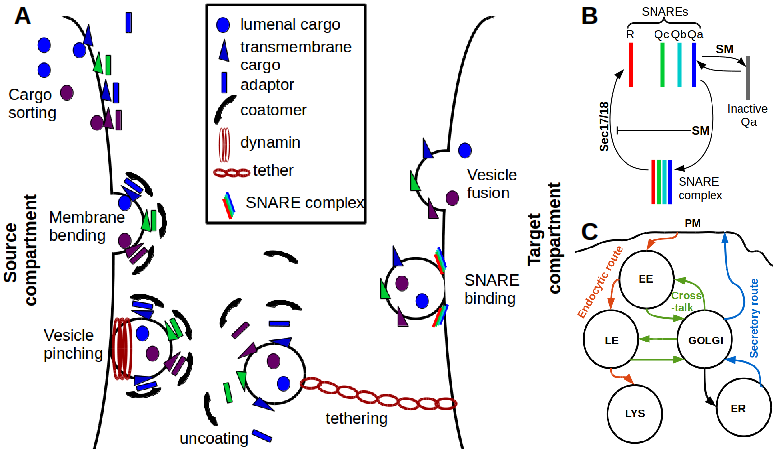
\includegraphics[height=9cm,width=12cm]{fig.png}
	\end{center}

	\caption{(A) Schematic of the vesicle transport system. Steps involved in vesicle transport between
		two compartments: a source and a target compartment, are shown. The symbols used for different
		molecules involved in vesicle traffic are explained in the key. At the source compartment,
		transmembrane cargo proteins are sorted by cytosolic adaptor proteins. Here, different colours
		indicate different types of cargo and adaptor proteins. Coat proteins are recruited to the forming
		vesicle by adaptor proteins. Note here that a single type of coat protein can interact with multiple
		types of adaptor proteins. Subsequently, the vesicle is pinched off at its neck, for example by dynamin
		protein. Once the vesicle has left the source compartment, the coat and adaptor proteins fall off and
		the vesicle is recognized and bound by a tethering complex which is linked to the target compartment.
		At the target compartment, the tethered vesicle undergoes fusion, thereby releasing its contents. (B)
		SNARE regulation network. Here, the dark blue, light blue, green and red stripes represent Qa, Qb,
		Qc and R SNAREs respectively. These 4 SNAREs interact to form a SNARE complex. SNARE
		complex formation is regulated by SM proteins and Sec 17/18. SM proteins inhibit SNARE complex
		formation by inactivating Qa SNAREs. They also enhance SNARE complex formation by stabilizing
		intermediate structures, and by inhibiting premature SNARE complex resolution. Sec17/18 aid in
		SNARE complex resolution. (C) A schematic of the typic eukaryotic cell's VTS. Large circles
		represent compartments, and edges represent vesicle routes. Identities of compartments are written
		inside or beside them; ER = endoplasmic reticulum, Golgi = Golgi apparatus, PM = plasma
		membrane, EE = early endosome, LE = late endosome, Lys = lysosome. The two major vesicle routes;
		the secretory and the endocytic routes are in blue and orange, respectively. The routes in green
		represent vesicles that allow cross-talk between the secretory and the endocytic routes. }
    \label{fig:vts}
\end{figure}

\subsubsection{Vesicle budding} 
The process of vesicle budding involves sorting and packaging of cargo molecules, membrane deformation and budding of the vesicle from the source compartment (Fig.~\ref{fig:vts}). 
%
Cargo sorting is performed by cytosolic adaptor proteins. 
%
Adaptor proteins bind to cargo molecules on the source
compartment and thereby sequester them for packaging \cite{paczkowski2015cargo}. 
%
Next, cytosolic coat proteins are recruited to the forming vesicle through their interaction with adaptor proteins \cite{faini2013vesicle}. 
%
Coat proteins cause membrane deformation. 
%
Finally, transport vesicles bud out from the source
compartment \cite{cocucci2014dynamin}. 
%
The vesicle is now ready for transport and subsequent fusion with a target compartment.
%
%The process of vesicle budding involves sorting and packaging of cargo molecules, membrane deformation and budding of the vesicle from the source compartment (Fig.~\ref{fig:vts}).
%%
%Cargo sorting is performed by cytosolic adaptor proteins. 
%Adaptors are recruited to the source compartment through interactions with the lipids that form the compartment's membrane, and interactions with molecular switches called Arf/Sar which signal the initiation of vesicle formation~\cite{paczkowski2015cargo}. 
%%
%Then these adaptors bind to cargo molecules and thereby sequester them for packaging. 
%%
%Different adaptor proteins act at different compartments, for example, vesicle formation at the ER requires the adaptor sec23/24, and the AP2 adaptor is used for packaging vesicles at the plasma membrane.
%%
%
%The next step is membrane deformation, which involves cytosolic coat proteins. 
%%
%Coat proteins are recruited to the forming vesicle through their interaction with adaptor proteins. 
%%
%These are naturally curved proteins, and their assembly on membranes leads to membrane deformation.
%%
%A single kind of coat protein can bind to multiple kinds of adaptors, thereby allowing the packaging of multiple types of cargo within the same vesicle. 
%%
%There are three major types of coat proteins: Clathrin, COP2, and COP1. These act on different compartments: the clathrin coat operates at multiple compartments, and can interact with multiple adaptors proteins, whereas the COP2 and COP1 coat are only involved in vesicle formation at a single compartment: the ER and the Golgi respectively~\cite{faini2013vesicle}.
%%
%Finally, transport vesicles bud out from the source compartment~\cite{cocucci2014dynamin}.
%%
%The vesicle is now ready for transport and subsequent fusion with a target compartment.

\subsubsection{Vesicle fusion} 
The process of vesicle fusion involves two steps: recognition of the correct target compartment and fusion of the transport vesicle (Fig.~\ref{fig:vts}). 
%
Target compartment recognition involves molecular
switches called Rabs and tethering complexes \cite{rink2005rab}. 
%
Rabs are master regulators; in their active form, Rabs recruit many downstream proteins, including tethering complexes, fusion regulators, motor proteins, etc, to their compartment \cite{muller2018molecular}. 
%
Tethering complexes sequester vesicles to their target compartments by binding to the vesicle on one end and the target compartment on the other end, thereby bridging the two
before fusion \cite{baker2016chaperoning}.

The final step in vesicle transport is the fusion of the vesicle with the target compartment is brought about by SNARE proteins. 
%
There are four kinds of SNAREs: R, Qa, Qb, and Qc; and vesicle fusion requires formation of a SNARE complex containing one of each type. 
%
In all known cases, one SNARE protein of the complex is contributed by the vesicle and the other three SNAREs by the target compartment. 
%
A few SNARE proteins, such as SNAP25, contain both Qb- and Qc-SNARE motifs~\cite{yoon2018snare}.

%\somya{schematic of snare regulatory network}
\subsubsection{Schematic of snare regulatory network}
In keeping with their central role in vesicle transport, both the activity and the localization of SNARE proteins are regulated. Notable regulators are Sec17/18 and the SM proteins.
%
Sec17/18 bring about disassembly of SNARE complexes post-fusion in order that these SNAREs may be reused. 
%
Whereas, SM proteins have following multiple modes of SNARE regulation: 
\begin{itemize}
	\item SM proteins can hold
	the Qa-SNAREs in an inhibited state and prevent or postpone their assembly into SNARE
	complexes.
	%
	\item Some SM proteins can act as a template upon which an early SNARE complex intermediate can form.
	%
	\item Finally, SM proteins bind the fully assembled
	SNARE complexes to protect them from premature disassembly by Sec17/18~\cite{baker2016chaperoning}.
	%
	\item SM proteins have also been shown to interact with tethers~\cite{yoon2018snare}.
\end{itemize}

%\somya{schematic of intracellular compartments and  major routes}
\subsubsection{Major paths in the VTS}
Molecules traverse the cell in a series of vesicles, and there are two major routes of vesicle transport in all eukaryotic cells.
%
\begin{itemize}
	\item The secretory route takes proteins from the ER (their site of production) to the plasma membrane (from where they are secreted out of the cell) via the Golgi apparatus~\cite{alberts2002molecular}.
	%
	\item The endocytic route takes proteins from the outside of the cell, through the plasma membrane, to the endocytic compartments and the lysosome where they are digested. 
\end{itemize}
Other paths are used for cross talk between the secretory and the endocytic routes. For example, vesicles are sent back and forth between the Trans-Golgi network (secretory route) to the early and the late endosomes (endocytic route)~\cite{progida2016bidirectional}. Also, recently, unconventional vesicle-mediated secretory routes have been found, which bypass the Golgi apparatus. The molecules involved in these routes are as yet unknown~\cite{nickel2018unconventional}. 
%
%\begin{table}
%	\begin{center}
%		\begin{tabular}{|c|c|c|c|c|c|c|c|c|c|c|}
%			\hline
%			Nodes & 1 & 2 & 3 & 4 & 5 & 6 & 7 & 8 & 9 & 10 \\ \hline
%			Graphs & 0 & 0 & 0 & 1 & 2 & 15 & 121 & 2159 & 68715 & 3952378 \\ 
%			\hline
%		\end{tabular}
%		\label{tab:threec}
%		\caption{Number of simple 3-edge-connected unlabelled N-node graphs.}
%	\end{center}	
%\end{table}

\subsection{The model}
\noindent The VTS model for this paper is inspired by~\cite{shukla2017discovering}. 
%
On the timescales of minutes, we have tried to capture important aspect of Rothman-Schekman-Sudhof (RSS) model~\cite{rothman2002machinery} of vesicle traffic system.
%
The following are the basic component and assumptions of our model. 
\begin{enumerate}
\item A cell is a set of compartments exchanging vesicles.
\item Compartments are neither created nor destroyed~\cite{braell1984glycoprotein}.
\item Each compartment is in steady state, gain and loss of the molecules is balance~\cite{braell1984glycoprotein}.
\item Molecules are neither created nor destroyed~\cite{he2009differential}.
\item Molecules move via vesicles of uniform size.
\item Identical vesicles have identical target compartments~\cite{fries1981transient}.
\item Fusion of vesicles to compartments is driven by specific SNARE pairing~\cite{mcnew2000compartmental}.
%\item The identities of compartments and vesicles is encoded in their molecules, and identical vesicles fuse with identical target compartments.
\item The activity of a SNARE can be regulated by other molecules present on the same compartment or vesicle~\cite{mima2008reconstituted}.
\item An active SNARE pair is necessary and sufficient for fusion~\cite{weber1998snarepins}
. 
\end{enumerate}
%
All our assumptions, except assumption 5, are held up by cell biological results.
%
Although vesicles produced in a cell do vary in size~\cite{jena2008intracellular}, they are much smaller than compartments, hence for the sake of simplicity, we assume a uniform size for intracellular vesicles.
%The assumptions 
%On the timescale of minutes, compartments are neither created nor destroyed, rather, they are in steady state. We assume that molecules are also neither created nor destroyed.
%The activity of a SNARE can be regulated by other molecules present on the same compartment or vesicle.

\subsection{Abstraction of VTS as a graph problem}

%In this section, we will describe the basic constraints imposed by cell biology. These are all incorporated into an abstract model of a VTS, whose properties will then be explored using SMT solvers.

\noindent In this section, we will abstract from the biological description of the VTS and represent the whole network as an annotated transport graph. 
%
The constraints imposed by cell biology are incorporated in the annotations of the graph. 

\subsubsection{The cell as a transport graph} 
%We consider a cell to be a collection of compartments (nodes) and vesicles (edges), thus defining a transport graph. Every compartment or vesicle has a set of molecular labels, such as SNARE proteins, associated with it.
The cell can be abstractly represented as an annotated graph. 
Every compartment in the cell can be represented as a node in the graph. 
%
The set of molecules present in the compartment, for example, SNARE proteins associated with it, are represented as a label to the corresponding nodes.
%
The label of each node will be unique molecules present on the compartment, i.e we abstract over the quantity of the molecule present in a compartment.
%This represents the flux of the molecule type present at that compartment.
%
The transport vesicle flowing from source compartment to the target compartment is represented by a labeled directed edge. 
% 
The label represents the associated flux of all molecular types carried by the corresponding vesicle.
%
%

\subsubsection{Steady state} 
The vesicle transfer will change the molecular composition (distinct molecule count) on both the source compartment and the target compartment. 
%
In our model, we assume that the cell is in a steady state. As a further simplification, we also assume that the incoming and outgoing flux is balanced for each of the molecular types at each compartment. 
Indeed, it is well accepted that on the scale of minutes and hours the molecular composition remains the same. 
%
In this paper, we refer to the steady state of the cell (referred to as \textit{homeostasis} in biological literature) as the stability condition over the annotated graph.


%Each edge is associated with a flux of all the molecular types carried by the corresponding vesicle. The total amount of each molecular type on each compartment can therefore increase or decrease. We assume the cell is in a steady state where each compartment’s composition does not vary over short time scales. Therefore, incoming and outgoing fluxes are balanced for each molecular type at each compartment; it is the \textit{stability cond1ition}.

\subsubsection{Vesicle fusion}
%Based on the earlier discussion of fusion, the vesicle targeting is driven by molecular interactions.  
%
%Particularly, molecules composition (SNARE proteins etc) present on the budded vesicle determines it's properties, which 
% 
%The molecular composition and hence the properties of the transfer vesicle 
%is the crucial factor to which target compartment the vesicle will fuse to.
%
%For any given pair of a vesicle and a compartment, the SNARE proteins present on both influence the fusion of the vesicle to that compartment.
%  
%Biophysically, fusion of a vesicle to the target compartment requires a direct physical interaction between at least one SNARE type on the vesicle and one SNARE type on the compartment.
%
%Once a vesicle has budded out of the source, the molecules it carries determine its properties. In particular, for any given pair of a vesicle and a compartment, the set of SNARE proteins that label the former and latter influence whether the vesicle will fuse to that compartment. Biophysically, fusion requires a direct physical interaction between at least one SNARE type on the vesicle and one SNARE type on the compartment. 
%
%SNAREs are of two types (known as Q and R in the cell biology iterature) and 
Vesicle fusion requires a pairing of 3 Q-SNAREs and 1 R-SNARE that are distributed between the transfer vesicle and the target compartment. 
%For any given pair of a vesicle and a compartment, vesicle fusion requires a pairing of a Q-SNARE with an R-SNARE on 
%the SNARE proteins present on both influence the fusion of the vesicle to that compartment.
%
%The list of molecular pairs that can drive a fusion event is given in a pairing matrix between Q and R SNAREs. 
%
Not all sets of Q and R-SNAREs are allowed to fuse with each other.
%
%In the model, we assume that the cell has an equal number of Q and R SNARE types.
%
Therefore, we can abstract the underlying cell biology by labeling the nodes and edges with Q and R-SNAREs. 
% equal number of Q and R SNAREs as a part of node and edge label.
%
%
Given a relation of all allowed fusion SNARE pairings, we can computationally determine whether a particular transfer vesicle will fuse to a particular target compartment (the edge between two compartments) based on the above condition.  

\subsubsection{Molecular regulation} 
Fusion takes place only if the SNARE types involved in the vesicle and compartment are both in an active state.
%We assume that for fusion to occur, the pair of 
%
The activity of these SNAREs is dependent on the presence of other molecules on the vesicle or compartment, respectively.
%
In our abstract model, 
we create a hierarchy of variants for varying degrees of regulation of SNARE activity.
%we create a set of variations of different kind of molecular regulations.
%
Most generally, the activity state of a given SNARE can be a Boolean function of all the molecular types on a compartment or vesicle. 
%
We have also tested \cite{shukla2017discovering} a particularly simple regulation mechanism in which two SNAREs that can pair to drive fusion to inhibit one another; this is the \textit{pairing inhibition}. 
%
This is motivated by the idea that pairing must generate an inactive bi-molecular complex.
%
Pairing inhibition can be encoded as a pairing matrix $P$, whose rows and columns represent the molecule types present in the VTS. 
%
$P(i,j)$ = 1 implies that molecule $i$ binds molecule $j$.
%
In our simple pairing inhibition scheme, if $P(i,j)$ = 1 and both molecules $i$ and $j$ are present on the same compartment, $i$ and $j$ are inactive, and therefore cannot cause fusion.

%We assume that for fusion to occur, the pair of SNARE types involved on the vesicle and compartment must both be in an active state. Whether these SNAREs are active or inactive depends on the other molecules found on the vesicle or compartment, respectively. We test many different versions of this kind of molecular regulation. Most generally, the activity state of a given SNARE can be a Boolean function of all the molecular types on a compartment or vesicle. We have also tested \cite{shukla} a particularly simple regulation mechanism in which two SNAREs that can pair to drive fusion inhibit one another; this is the \textit{pairing inhibition}. This is motivated by the idea that pairing must generate an inactive bi-molecular complex.

%\textbf{Difficulty of the analysis:}

%
%Properties of the VTS would be hindered by the same reason. 
%3-connected graphs and all possible variations of SNARE regulation rules. 
%
%The number of graphs of specified connectivity grows exponentially with the number of nodes: Table~\ref{tab:threec} shows how many 3-edge-connected graphs~\cite{a052448-oeis} exist (without parallel or self edges) as node number N increases.
\subsection{Graph connectivity is an interesting and accessible property of the VTS} 
%\textbf{Properties of a VTS that satisfies all cell-biological constraints:} 
%\noindent Interactions between the molecules of the VTS together produce a functional vesicle transport network, in which molecules flow between intracellular compartments using specified paths.
%%
%The molecules of the VTS, their interactions, and modes of regulation have been worked out to a large extent through cell-biological experiments. 
%%
%But we do not know if this information is complete. In order to assess how completely we know the VTS, we need easily readable benchmarks. 
%
%One such benchmark is provided by our result about the connectivity of the VTS graph. Graph connectivity is defined as the minimum number of edges that need to be removed from an undirected graph to render it disconnected. 
%\textbf{Properties of a VTS that satisfies all cell-biological constraints:} 
Suppose we are given a particular transport graph, a particular labeling of all the compartments and edges, a particular fusion pairing matrix, and a particular regulatory model. This information is then sufficient to check the following properties, which summarise the cell-biological constraints described above:
\begin{enumerate}
	\item We can determine which molecules are active on every compartment or vesicle.
	\item For every vesicle fusing to a compartment, we can determine whether there exists an active pair (one molecule on the vesicle, one on the compartment) which drives that fusion event.
	\item For every vesicle-compartment pair where the vesicle does not fuse to the compartment, we can verify that there is no pairing of active molecules on the
	vesicle and compartment that could drive their fusion.
	\item We can verify that every molecular type entering a compartment also leaves the compartment, and also that every molecular type entering a set of compartments also leaves that set. This is the steady state condition. In the biological literature this is often referred to as “homeostasis” and is a widespread and well-accepted assumption about cellular behaviour, at least over timescales of minutes to hours \cite{mani2016stacking}.
\end{enumerate}

The biological problem often boils down to such an analysis. A cell biologist might determine which molecules flow between which set of compartments, and biochemical experiments could be used to see how these molecules activate one another. We can then ask: is this a complete and consistent description? That is, do all the required properties listed above hold, given what the experimentalists have told us? It is often the case that biological data is missing. For example, only a few of the dozens of molecules involved in real VTSs have been mapped out. Therefore, it is extremely likely that the description provided by the cell biologist is incomplete. We can use our model to find out which properties have failed to hold, and thus prescribe new experiments in order to fill in the missing information.

Can we find a simple test to see whether any information is missing, given the experimental data? It has shown that graph k-connectedness furnishes precisely such a test \cite{shukla2017discovering}.
%
If the data provided by cell-biologists, suitably represented as a graph, does not have a certain degree of connectivity, this implies that some biological data has been missed. (The converse is not true: even if the required connectivity does hold, there might of course be more information missing.)

%The result about k-connectedness being a useful test of missing information \cite{shukla2017discovering} was obtained using SAT solvers for graphs up to a certain size, and a certain number of molecules. This was due to limitations in how we encoded the problem. Here we present a much more natural encoding that allows our result to be extended to graph sizes and molecule numbers that are typical of those found in real cells.


%For example, in a directed cyclic graph, every node has at least one incoming and one outgoing edge, at least 2 edges need to be removed in order to disconnect the graph. Therefore the underlying undirected graph is 2-connected. 
%From our result, for a given set of biomolecular interactions, for a cell that is in a steady state, we expect the VTS graph to have a certain k-connectivity. When regulation is given by arbitrary Boolean rules, we find that VTS graphs must be 3-connected. And when we add the constraint of the specific form of regulatory interactions seen between VTS molecules, we expect vesicle transport graphs to be 2 strongly connected.

%\ankit{We need not specify Synthesis here. Only connectivity use next subsection to build this.}
%\somya{But this is the para where we explain why connectivity is interesting an biological property}
%\ankit{Yes; Both of our remark looks correct!}
%The vesicle transport graphs available today for eukaryotic organisms are incomplete themselves. 
%%
%In this situation, we use our result as a tool to predict missing edges which satisfy the graph connectivity constraint. 
%%
%These predictions are intended to be used as guides for future experiments. 
%%
%A mismatch between our predictions and experiments would indicate that our current understanding of the VTS molecules is necessarily incomplete. 
%%
%Note that, on the other hand, if our predictions are experimentally confirmed, it does not imply that our understanding of the VTS is complete.\\
%%
%\begin{table}[!t]
%	\caption{Table Caption}
%	\label{tab1}
%	\centering
%	{\setlength\tabcolsep{0.1pt}%
%		\begin{tabular}{ccccccccccccccc}
%			& $D_1$ & $D_2$ & $D_3$ & $D_4$ & $D_5$ & $D_6$ && & $D_1$ & $D_2$ & $D_3$ & $D_4$ & $D_5$ & $D_6$ \\
%			$D_1$ & & \cca{0} & \cca{0} & \cca{0} & \cca{2} & \cca{0} && $D_1$ && \cca{0} & \cca{0} & \cca{2} & \cca{2} & \cca{2} \\
%			$D_2$ & \cca{0} & & \cca{2} & \cca{0} & \cca{2} & \cca{0} && $D_2$ & \cca{0} &  & \cca{3} & \cca{0} & \cca{0} & \cca{2} \\
%			$D_3$ & \cca{7} & \cca{4} &  & \cca{3} & \cca{0} & \cca{4} && $D_3$ & \cca{0} & \cca{4} &  & \cca{4} & \cca{2} & \cca{0} \\
%			$D_4$ & \cca{3} & \cca{0} & \cca{7} &  & \cca{4} & \cca{0} && $D_4$ & \cca{0} & \cca{0} & \cca{5} &  & \cca{0} & \cca{0} \\
%			$D_5$ & \cca{3} & \cca{7} & \cca{7} & \cca{2} &  & \cca{4} && $D_5$ & \cca{2} & \cca{2} & \cca{0} & \cca{4} &  & \cca{4} \\
%			$D_6$ & \cca{2} & \cca{2} & \cca{7} & \cca{2} & \cca{6} &  && $D_6$ & \cca{2} & \cca{2} & \cca{3} & \cca{0} & \cca{4} & \\
%	\end{tabular}}
%\end{table}
%
\begin{figure}[t]
\centering
  \begin{subfigure}[b]{\linewidth}
   \centering
 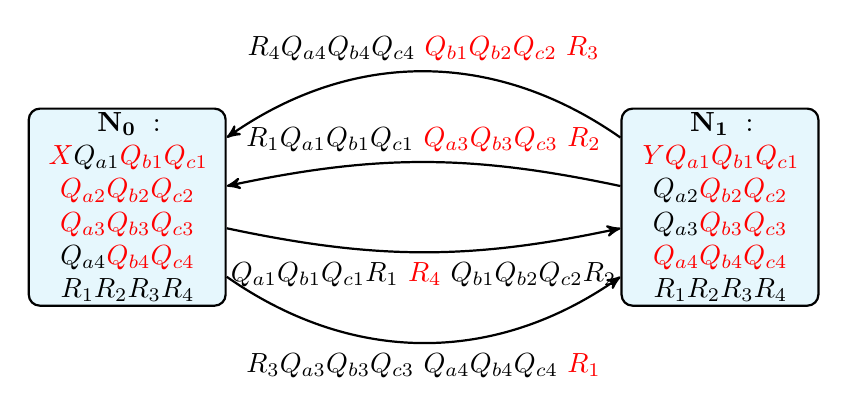
\begin{tikzpicture}[node distance=3.3cm and 5cm,->,>=stealth', auto,thick ] 
\tikzset{
	rc/.style={rounded corners=2mm,line width=0.5pt},
	%
	place/.style={draw,rectangle,fill=cyan!10,inner sep=.5mm,minimum size=3mm, text width=2.4cm,rounded corners,align=center},
}
 \node[state,place](a) {$\mathbf{N_{0}}: {\color{red}X} Q_{a1}  \color{red}Q_{b1} Q_{c1}$ $\color{red}Q_{a2} Q_{b2} {\color{red}Q_{c2}}$ $\color{red}Q_{a3} Q_{b3} Q_{c3}$ $Q_{a4} \color{red}Q_{b4} Q_{c4}$ $R_{1} R_{2} R_{3} R_{4}$};
 \node[state,place,right=of a] (b) {$\mathbf{N_{1}}: {\color{red}Y} \color{red} Q_{a1} Q_{b1} Q_{c1}$ $Q_{a2} \color{red}Q_{b2} Q_{c2}$ $Q_{a3} \color{red}Q_{b3} Q_{c3}$ $\color{red}Q_{a4} Q_{b4} Q_{c4}$ $R_{1} R_{2} R_{3} R_{4}$};  
 \draw
 (a) edge[bend right=12,auto=right,->] node[auto]{$Q_{a1} Q_{b1} Q_{c1} R_{1}$  $\color{red}R_{4}$ $Q_{b1} Q_{b2} Q_{c2} R_{2}$} (b)  
  (a) edge[bend right=35,auto=right,->] node[auto] {$R_{3} Q_{a3} Q_{b3} Q_{c3}$  $Q_{a4} Q_{b4} Q_{c4}$ $\color{red}R_{1}$} (b)  
  (b) edge[bend right=12,auto=right,->] node[auto] {$R_{1} Q_{a1} Q_{b1} Q_{c1}$ $\color{red}Q_{a3} Q_{b3} Q_{c3}$ $\color{red}R_{2}$} (a)
 (b) edge[bend right=35,auto=right,->] node[auto] {$R_{4} Q_{a4} Q_{b4} Q_{c4}$ $\color{red}Q_{b1} Q_{b2} Q_{c2}$ $\color{red}R_{3}$}  (a);  
 \end{tikzpicture}
 
%\begin{tikzpicture}[node distance=3.3cm and 5cm,->,>=stealth', auto ]
%\tikzset{
%	sh2n/.style={shift={(0,1)}},
%	sh2s/.style={shift={(0,-1)}},
%	sh2e/.style={shift={(1,0)}},
%	sh2w/.style={shift={(-1,0)}},
%	%
%	sh2nw/.style={shift={(-1,1)}},
%	sh2ne/.style={shift={(1,1)}},
%	sh2sw/.style={shift={(-1.5,-1)}},
%	sh2se/.style={shift={(1,-1)}},
%	sh2sm/.style={shift={(0.5,-1.8)}},
%	%
%	rc/.style={rounded corners=2mm,line width=0.5pt},
%	%
%	place/.style={draw,rectangle,fill=cyan!10,inner sep=.5mm,minimum size=5mm, text width=3.0cm,rounded corners,align=center},
%}
%%$Q_{a1} {\color{red} Q_{b1}} Q_{c1}, \color{red}Q_{a2} Q_{b2}$ ${\color{red}Q_{c2} Q_{a3} Q_{b3} Q_{c3}} Q_{a4}$ $Q_{b4} Q_{c4} R_{1} R_{2} R_{3} R_{4}$
%\node[place] (a) {$Node_{1}:$ $Q_{a1} {\color{red} Q_{b1}} Q_{c1}$ $\color{red}Q_{a2} Q_{b2} {\color{red}Q_{c2}}$ $Q_{a3} Q_{b3} Q_{c3}$ $Q_{a4} Q_{b4} Q_{c4}$ $R_{1} R_{2} R_{3} R_{4}$};
%\node[place,left=of a] (b) {$Node_{0}:$ $Q_{a1} {\color{red} Q_{b1}} Q_{c1}$ $\color{red}Q_{a2} Q_{b2} {\color{red}Q_{c2}}$ $Q_{a3} Q_{b3} Q_{c3}$ $Q_{a4} Q_{b4} Q_{c4}$ $R_{1} R_{2} R_{3} R_{4}$};
%%\node[place,left=of a] (b) {$Node_{0}:$ ${\color{red}Q_{a1} Q_{b1} Q_{c1}} Q_{a2} Q_{b2}$ $Q_{c2} Q_{a3} Q_{b3} Q_{c3} \color{red}Q_{a4}$ ${\color{red}Q_{b4} Q_{c4}} R_{1} R_{2} R_{3} R_{4}$};
%%\node[place,above right=of a] (c) {c};
%
%\draw[-stealth,rc] (a) -- node[above]{$Q_{a1} Q_{b1} Q_{c1} R_{1}$  $\color{red}R_{4}$} node[below,pos=.35] {$Q_{b1} Q_{b2} Q_{c2} R_{2}$} (b);
%%\draw[-stealth,rc] (a) |- node[green!50!black,above,pos=.75]{a to c} (c);
%\draw[-stealth,rc] (a) -- ([sh2nw]a.center) -- node[above] {$R_{3} Q_{a3} Q_{b3} Q_{c3}$  $Q_{a4} Q_{b4} Q_{c4}$ $\color{red}R_{1}$} ([sh2n]b.center) -- (b);
%%\draw[-stealth,rc] (b) -- ([sh2nw]a.center) -- node[above,red] {} ([sh2n]b.center) -- (a);
%\draw[-stealth,rc] (b) -- ([sh2se]b.center) -| node[above,pos=.25] {$R_{1} Q_{a1} Q_{b1} Q_{c1}$} node[below,pos=.25] { $\color{red}Q_{a3} Q_{b3} Q_{c3}$ $\color{red}R_{2}$} (a);
%\draw[-stealth,rc] (b) -- ([sh2sm]b.center) -| node[below,pos=.25] {$R_{4} Q_{a4} Q_{b4} Q_{c4}$ $\color{red}Q_{b1} Q_{b2} Q_{c2}$ $\color{red}R_{3}$} (a);
%\end{tikzpicture}
 % \caption{VTS as an annotated graph}
\end{subfigure}

\vspace{0.7cm}
  \begin{subfigure}[b]{\linewidth}
  \centering
  \resizebox{0.8\textwidth}{!}{
  \begin{tabular}{p{0.5cm}|p{0.2cm}p{0.2cm}p{0.2cm}p{0.2cm}p{0.2cm}p{0.2cm}p{0.2cm}p{0.2cm}p{0.2cm}p{0.2cm}p{0.2cm}p{0.2cm}p{0.2cm}p{0.2cm}p{0.2cm}p{0.2cm}p{0.2cm}p{0.2cm}}

%                \cline{2-17}\hline
				& $X$ & $Y$ &$Q_{a1}$ & $Q_{b1}$ & $Q_{c1}$ &  $Q_{a2}$ & $Q_{b2}$ & $Q_{c2}$ &  $Q_{a3}$ & $Q_{b3}$ & $Q_{c3}$ &  $Q_{a4}$ & $Q_{b4}$ & $Q_{c4}$ & $R_{1}$ & $R_{2}$ & $R_{3}$  & $R_{4}$ \\
				  	\cline{2-17} \hline
				$X$ &  \cca{0} & \cca{0} & \cca{0} & \cca{0} & \cca{0} & \cca{1} & \cca{0} & \cca{0} & \cca{0} & \cca{1} & \cca{0} & \cca{0} & \cca{0}  & \cca{0} & \cca{0} & \cca{0}  & \cca{0}  & \cca{0} \\
				$Y$ & \cca{0} & \cca{0} & \cca{1} & \cca{0} & \cca{0} & \cca{0} & \cca{0} & \cca{0} & \cca{0} & \cca{0} & \cca{0} & \cca{1} & \cca{0}  & \cca{0} & \cca{0} & \cca{0}  & \cca{0}  & \cca{0} \\
				$Q_{a1}$ & \cca{0} & \cca{1} & \cca{0} & \cca{1} & \cca{1} & \cca{0} & \cca{0} & \cca{0} & \cca{0} & \cca{0} & \cca{0} & \cca{0} & \cca{0}  & \cca{0} & \cca{1} & \cca{0}  & \cca{0}  & \cca{0}\\
				$Q_{b1}$ &  \cca{0} & \cca{0} & \cca{1} & \cca{0} & \cca{1} & \cca{0} & \cca{0} & \cca{0} & \cca{0} & \cca{0} & \cca{0} & \cca{0} & \cca{0}  & \cca{0} & \cca{1} & \cca{0}  & \cca{0}  & \cca{0} \\
				$Q_{c1}$ &  \cca{0} & \cca{0} & \cca{1} & \cca{1} & \cca{0} & \cca{0} & \cca{0} & \cca{0} & \cca{0} & \cca{0} & \cca{0} & \cca{0} & \cca{0}  & \cca{0} & \cca{1} & \cca{0}  & \cca{0}  & \cca{0} \\
				$Q_{a2}$ & \cca{1} & \cca{0} &  \cca{0} & \cca{0} & \cca{0} & \cca{0} & \cca{1} & \cca{1} & \cca{0} & \cca{0} & \cca{0} & \cca{0} & \cca{0}  & \cca{0} & \cca{0} & \cca{1}  & \cca{0}  & \cca{0} \\
				$Q_{b2}$ & \cca{0} & \cca{0} & \cca{0} & \cca{0} & \cca{0} & \cca{1} & \cca{0} & \cca{1} & \cca{0} & \cca{0} & \cca{0} & \cca{0} & \cca{0}  & \cca{0} & \cca{0} & \cca{1}  & \cca{0}  & \cca{0} \\
				$Q_{c2}$ & \cca{0} & \cca{0} & \cca{0} & \cca{0} & \cca{0} & \cca{1} & \cca{1} & \cca{0} & \cca{0} & \cca{0} & \cca{0} & \cca{0} & \cca{0}  & \cca{0} & \cca{0} & \cca{1}  & \cca{0}  & \cca{0} \\
				$Q_{a3}$ & \cca{1} & \cca{0} & \cca{0} & \cca{0} & \cca{0} & \cca{0} & \cca{0} & \cca{0} & \cca{0} & \cca{1} & \cca{1} & \cca{0} & \cca{0}  & \cca{0} & \cca{0} & \cca{0}  & \cca{1}  & \cca{0} \\
				$Q_{b3}$ & \cca{0} & \cca{0} & \cca{0} & \cca{0} & \cca{0} & \cca{0} & \cca{0} & \cca{0} & \cca{1} & \cca{0} & \cca{1} & \cca{0} & \cca{0}  & \cca{0} & \cca{0} & \cca{0}  & \cca{1}  & \cca{0} \\
				$Q_{c3}$ & \cca{0} & \cca{0} & \cca{0} & \cca{0} & \cca{0} & \cca{0} & \cca{0} & \cca{0} & \cca{1} & \cca{1} & \cca{0} & \cca{0} & \cca{0}  & \cca{0} & \cca{0} & \cca{0}  & \cca{1}  & \cca{0} \\
				$Q_{a4}$ & \cca{0} & \cca{1} & \cca{0} & \cca{0} & \cca{0} & \cca{0} & \cca{0} & \cca{0} & \cca{0} & \cca{0} & \cca{0} & \cca{0} & \cca{1}  & \cca{1} & \cca{0} & \cca{0}  & \cca{0}  & \cca{1} \\
				$Q_{b4}$ & \cca{0} & \cca{0} & \cca{0} & \cca{0} & \cca{0} & \cca{0} & \cca{0} & \cca{0} & \cca{0} & \cca{0} & \cca{0} & \cca{1} & \cca{0}  & \cca{1} & \cca{0} & \cca{0}  & \cca{0}  & \cca{1} \\
				$Q_{c4}$ & \cca{0} & \cca{0} & \cca{0} & \cca{0} & \cca{0} & \cca{0} & \cca{0} & \cca{0} & \cca{0} & \cca{0} & \cca{0} & \cca{1} & \cca{1}  & \cca{0} & \cca{0} & \cca{0}  & \cca{0}  & \cca{1} \\
				$R_{1}$ & \cca{0} & \cca{0} & \cca{1} & \cca{1} & \cca{1} & \cca{0} & \cca{0} & \cca{0} & \cca{0} & \cca{0} & \cca{0} & \cca{0} & \cca{0}  & \cca{0} & \cca{0} & \cca{0}  & \cca{0}  & \cca{0} \\
				$R_{2}$ &  \cca{0} & \cca{0} & \cca{0} & \cca{0} & \cca{0} & \cca{1} & \cca{1} & \cca{1} & \cca{0} & \cca{0} & \cca{0} & \cca{0} & \cca{0}  & \cca{0} & \cca{0} & \cca{0}  & \cca{0}  & \cca{0} \\
				$R_{3}$ & \cca{0} & \cca{0} & \cca{0} & \cca{0} & \cca{0} & \cca{0} & \cca{0} & \cca{0} & \cca{1} & \cca{1} & \cca{1} & \cca{0} & \cca{0}  & \cca{0} & \cca{0} & \cca{0}  & \cca{0}  & \cca{0} \\
				$R_{4}$ & \cca{0} & \cca{0}  & \cca{0} & \cca{0} & \cca{0} & \cca{0} & \cca{0} & \cca{0} & \cca{0} & \cca{0} & \cca{0} & \cca{1} & \cca{1}  & \cca{1} & \cca{0} & \cca{0}  & \cca{0}  & \cca{0}
				%\hline
  \end{tabular}
  }
 % \caption{Pairing matrix}
\end{subfigure}
\caption{An example of VTS and its corresponding pairing matrix. The compartments (node $N_0$, $N_0$) and vesicles (edges between nodes) are labeled with the present molecules. Present but inactive molecules are shown in black color whereas active molecules are shown in red. The pairing matrix of the VTS is shown below. Entry 1 between molecule $i$ and $j$ in the pairing matrix implies that molecule $i$ can bind with molecule $j$.} \label{fig:M1}
\end{figure}

%%% Local Variables:
%%% mode: latex
%%% TeX-master: "main"
%%% End:

%
\begin{example}
%
In Fig.~\ref{fig:M1}, we present a VTS that has 2 compartments and 18 molecules with its corresponding pairing matrix.
%
%Molecules are represented as $Q_{i}$'s or $R_{i}$'s to make a clear distinction between Q and R SNAREs.
%
In the VTS, labels are a set of molecule, where we show active molecules in red color.
%
The activity of the molecules on the node is controlled
by the presence of the other molecules (exact Boolean function is not shown). 
%
The activity of the molecules on an edge is determined by the corresponding pairing matrix.
%
Note that molecules $X$ and $Y$ do not take part in the fusion but determine the activity of molecules at the corresponding nodes.
%
Below the VTS, we show the pairing matrix.
%
Rows in the matrix correspond to the labels of edges, and columns correspond to the labels of nodes.
%
An entry 1 represents pairing between molecules and 0 represents no pairing.
%
Every molecule flows on a cycle, ensuring steady state.
%
This is a 4-connected graph.
\end{example}
\begin{figure}[t]
	\centering
	%\begin{minipage}{0.45\linewidth
 \begin{subfigure}[b]{0.49\linewidth}
%\begin{tikzpicture}[node distance = 30mm]

%\begin{tikzpicture}[->,>=stealth',shorten >=1pt,auto,node distance=2cm,
%thick,main node/.style={circle,draw,font=\sffamily,minimum size=0.8cm}]
%\begin{scope}[]
%
%\node[main node] (1) {$s_{1}$};
%\node[main node] (2) [below left of=1] {$s_{2}$};
%\node[main node] (3) [below right of=1] {$s_{3}$};
%
%\path[every node/.style={font=\sffamily\small}]
%(3) edge node [left] {} (1)
%(1) edge [loop above] node {} ()
%(2) edge [loop above] node {} ()
%(1) edge node [right] {} (2)
%(2) edge node[right] {} (3)
%(3) edge[bend left, below] node{} (2);
%%(3) edge [bend right] node[right] {} (2)
%\end{scope}
 \begin{tikzpicture}[->,>=stealth', auto , node distance=3.1cm,
	  thick,main node/.style={rectangle,draw,rounded corners}]
	 % 	\begin{scope}[]
	  \node[main node, text width=1.5cm] (pm) {$\mathbf{N_{0}}$: { {$Q_{a5}$} 
	  		                     {$Q_{a7}$} {$Q_{bc2}$} {$Q_{bc7}$}} ...};
	  \node[main node, text width=1.5cm] (ee) [below right of=pm] {$\mathbf{N_{1}}$: { {$Q_{a2}$} {$ Q_{b2/3} $} {$ Q_{c2/3} $}} ...};
	  \node[main node, text width=1.3cm] (le) [above of=ee,yshift=-10mm,xshift=20mm] {$\mathbf{N_{2}}$: { {$Q_{a8}$} {$Q_{b8}$} {$Q_{c8}$}} ...};
	
	  %le <-> pm
	  \path (le) edge[bend right=55] node [above] {$Q_{bc7}$} (pm);
	  \path (ee) edge[bend right=32, text width=1.8cm] node [below,right=0.1] {{$R_{8}$}, $Q_{a7}$, $Q_{bc7}$, $R_{7}$} (le);
	
	  %pm <-> ee
	  \path (ee) edge[bend left=32] node [below] {{$R_{3}$}} (pm);
	  \path (pm) edge[bend left=30, text width=2.1cm] node [above,rotate=-45] {{$R_{2}$}, {$Q_{a7}$}, $Q_{bc7}$, $R_{7}$, $Q_{a2}$} (ee);
	\end{tikzpicture}
	\caption{Input partial VTS} 
		 \label{fig:synth-vts1}
  \end{subfigure}%
 % \end{scope}
%  \vspace{1.2cm}
  \begin{subfigure}[b]{0.49\linewidth}
	  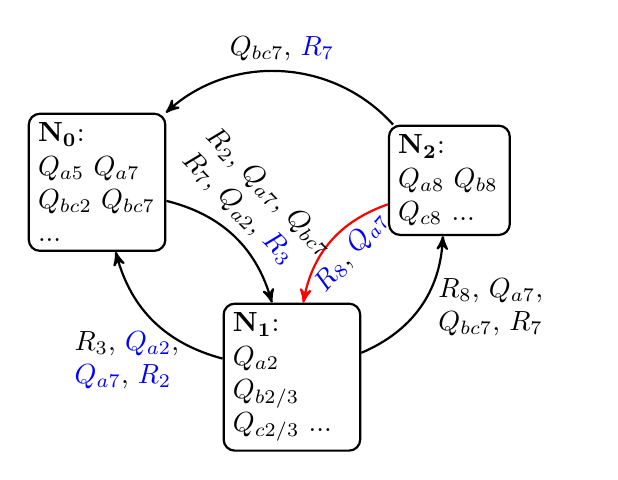
\begin{tikzpicture}[->,>=stealth',auto,node distance=3.5cm,
	  thick,main node/.style={rectangle,draw,rounded corners}]
	 % \begin{scope}[xshift=3.5cm,yshift=0.0cm]
	  \node[main node, text width=1.5cm] (pm) {$\mathbf{N_{0}}$: { {$Q_{a5}$} 
	  	  		                     {$Q_{a7}$} {$Q_{bc2}$} {$Q_{bc7}$}} ...};
	  	  \node[main node, text width=1.5cm] (ee) [below right of=pm] {$\mathbf{N_{1}}$: { {$Q_{a2}$} {$ Q_{b2/3} $} {$ Q_{c2/3} $}} ...};
	  	  \node[main node, text width=1.3cm] (le) [above of=ee,yshift=-10mm,xshift=20mm] {$\mathbf{N_{2}}$: { {$Q_{a8}$} {$Q_{b8}$} {$Q_{c8}$}} ...};
	  
	  %le <-> pm
	  	  \path (le) edge[bend right=45] node [above] {$Q_{bc7}$,{\color{blue}{ \textbf{$R_{7}$}}}} (pm);
	%  \path (le) edge[bend right=45] node [above] {Qb7 Qc7,{\color{blue} { \textbf{R7}}}} (pm);
	  
	  %le <-> ee
	  {\color{red} { \path (le) edge[bend right] node [below,rotate=50] {{\color{blue} { {\textbf{{$R_{8}$}}}}}{\color{black},} {\color{blue} {$Q_{a7}$}}} (ee);
	  }}
	  %ee -> le
	   \path (ee) edge[bend right=32, text width=1.8cm] node [below,right=0.1] {{$R_{8}$}, $Q_{a7}$, $Q_{bc7}$, $R_{7}$} (le);
%	  \path (ee) edge[bend right] node [text width=1.5cm, below,rotate=50] {{R8}, Qa7, Qbc7,R7} (le);	  
	  
	  %pm <-> ee
	  \path (ee) edge[bend left=30] node [below, text width=2.0cm] {{$R_{3}$,{\color{blue} { \textbf{{$Q_{a2} $}}}}, \\ {\color{blue} {{ $ Q_{a7}$}}}, {\color{blue} {{$R_{2}$}}}}} (pm);
	   \path (pm) edge[bend left=30, text width=2.3cm] node [above,rotate=-45] {{$R_{2}$}, {$Q_{a7}$}, $Q_{bc7}$ $R_{7}$, $Q_{a2}$, \color{blue} {$R_{3}$}} (ee);
%	  \path (pm) edge[bend left=30] node [above,rotate=-45,text width = 2.5cm] {{R2} {Qa7} Qbc7, R7, Qc7, Qa2, \color{blue} { \textbf{R3}}} (ee);	    
	 % \end{scope}

	 \end{tikzpicture}
	 \caption{Output complete VTS} 
	 \label{fig:synth-vts2}
  \end{subfigure}%
  \caption{An example of synthesis of edge and molecules in the partial VTS} \label{fig:synth-vts}
\end{figure}

  

\begin{example}
	In Fig.~\ref{fig:synth-vts1}, we present a partial input VTS that has 3 compartments. Fig.~\ref{fig:synth-vts2} present it's complete output VTS. Every molecule present on the node is active. The activity of the molecules on an edge is determined by the presence of the other molecules. Each label represent particular type of molecule. The synthesis is performed against the stability and 3-connectivity. Synthesized edge is in red color and synthesized molecules are presented in blue. The synthesis adds one edge and 7 molecules to complete the partial VTS. For the sake of clarity, we have not presented the activity of molecules, the corresponding pairing matrix and remaining molecules on the nodes. This synthetic example is a sub-graph of the VTS shown in the \ref{fig:mukund-vts}. Please refer to \ref{sec:ex-vts} for complete detail. 
	%The presented graph is a subgraph of a VTS discussed in details in appendix.
\end{example}

%
%\subsection{Modeling and Symbolic Analysis of VTS: An Overview}
\label{subsec:graphmodel}
%
%\subsection{Combinatorial problem and use of Formal methods}
%\noindent 
%The analysis of VTS is a difficult problem
%because of the combinatorial scaling of possible traffic topologies and regulatory rules. 
%
%For example, we might want to check some conjecture of interest for all graphs of a certain structure. 
%
%If the analysis is done on a large number of graphs, the joined effect of large quantity of graphs and combinatorially many possible regulatory rules will be difficult to handle by any tool

\subsubsection{Size of the VTS system}
%Let us discuss the rough sizes of the system and expected behaviors.
%%
%A typical VTS may have about 10 compartments.
%%
%%Across eukaryotes, there are 20 broad SNARE varieties, though individual species can
%%contain higher numbers (humans have 41)~\cite{kloepper2007elaborate}..
%%
%The VTS may transport a large number of molecules but the molecules that
%are relevant of the control of VTS are about 50~\cite{kloepper2007elaborate}.
%%
%According to the definition the activity of molecules can be controlled by
%the presence of all other molecules.
%%
%However, in practice the activity of a molecule is controlled by
%the presence of ~2-3 other molecules.
A typical eukaryotic cell contains 9 organelles; the ER, the cis-, medial- and trans-Golgi, the early, late and recycling endosomes, the lysosome and the plasma membrane~\cite{lodish2008molecular}. 
%
The organellar content of cells varies across different organisms, for example, parasitic cells such as Trypanosomes have specialized secretory organelles called rhoptries and micronemes~\cite{gubbels2012evolution}. 
%
The organellar content may also vary across different states of the same cell, for e.g., during cell division, the Golgi apparatus disintegrates into vesicles~\cite{tang2013cell}. 
%
Also, across different cell-types, these organelles may be more or less differentiated, for example, the number of stacks in the Golgi varies across different cells~\cite{polishchuk2004structural}. 
%

Going by the above description, we can assume that the VTS has of the order of 10 compartments. 
%
The VTS transports a large number of molecules but the molecules that actively control the system are in their tens~\cite{lodish2008molecular}. 
%
By definition, the activity of any VTS molecules can be controlled by all other molecules.
%
However, in practice the activity of a molecule is directly controlled by 2-3 other molecules; for example, adaptor proteins are recruited to compartments by lipids of the compartment membrane and by ARF/SAR GTPases~\cite{kahn2009toward}. 
%
Some molecules, such as Rab GTPases are master regulators which control many different VTS molecules with diverse functions~\cite{zerial2001rab}. 
%
But most VTS molecules have more localized influence.
%
We use the above information during the encoding of all search problems presented later.

% i.e., formally as a boolean function that given requisite labels of nodes and vesicles that returns true if the required regulations are met. 
%
%
% Note that the formulas define among other things constraints over
% paths between nodes in the graph model of VTS. Similarly, one can
% define fusion rules as constraints over the boolean functions modeling
% the regulations.  
% For example, the steady state condition, described informally earlier, can be defined by the formula shown in Listing~1.1.
%\begin{itemize}
%\item \srivas{Detailed BIO to Graph problem}
%\end{itemize}
%Given definitions of fusion and budding rules and the steady state conditions, whether a VTS meets maximum connectivity requirement, i.e. the LGC property, can be verified by checking if the formula show in Listing~1.2 is valid.  Here we have defined the property by checking over existence of any fusion/budding rules.  We can eliminate the existential quantifier if we are interested in checking the property for a particular fusion/budding rule.
%
%\subsection{Converting the Graph Problem into Boolean SAT problem}
%\label{subsec:satproblem}
%To convert the graph problem described in sec~\ref{subsec:graphmodeling}, into a boolean SAT problem, we need to define a scheme to represent graphs and boolean functions using a suitable set of propositional variables.  In our earlier work, we modeled the graph problem in C using arrays to model graphs and boolean function.  We then used the CBMC model checker to convert the graph problem into a SAT problem.  One of the challenges we had in our earlier work is dealing with quantifiers.  Note that the connectedness property defined in Listing~1.2 has quantifier alternation.  Even if we were to eliminate the existential quantifier by instantiating the problem for a fixed set of fusion rules, we would have embedded quantifiers in the antecedent of implications.   CBMC supports only a quantifier-free logic n its assertion language.  In our earlier work we used a combination of explicit enumeration at the C-level and clever use f non-determinism to eliminate alternation of quantifiers.  This enumeration was one source of bottleneck for scaling in our earlier work.  In the current work we eliminate this bottleneck by modeling the problem directly as a SAT instance using uninterpreted functions and recursive relations.  The details of te hnew encding will described in subsequent sections.
%A VTS is {\em $k$-connected} if every pair of compartments remain reachable after dropping $k-1$ vesicles.
%
%This property of VTSs has been considered informative and studied by~\cite{shukla}.
%
%Here we have build an {\em efficient} tool that studies properties of VTSs that are not $k$-connected, from some $k$. 
%\subsection{Synthesis of VTS }


%

%
%%% Local Variables:
%%% mode: latex
%%% TeX-master: "main"
%%% End:
~        

%\clearpage
\section{Preliminary}
\label{sec:prelim}
In this section, we will present the model of VTS from~\cite{smtVTS}.
%
We will also present the constrains and properties on the VTSs, and their
encoding as a QBF formula.   
%
We model a VTS as labelled graph along with assisting pairing matrices and
activating functions.

\begin{df}
  A VTS $G$ is a tuple $(\nodes,\mols,\edges,\nlabel,\pairs,\edgef,\nodef)$, where
  \begin{itemize}
  \item $\nodes$ is a set of nodes representing compartments in the VTS,
  \item $\mols$ is the set of molecules flowing in the system, 
  \item $\edges \subseteq \nodes \times (\powerset{\mols}-\emptyset) \times \nodes$ is the
    set of edges with molecule sets as labels,
  \item $\nlabel : \nodes \maps \powerset{\mols}$ defines the molecules present in the nodes,
  \item $\pairs \subseteq 2^{\mols}$ is pairing relation,
  \item $\nodef : \mols \maps \powerset{\mols} \maps \booleans$ is activity maps for nodes, and
  \item $\edgef : \mols \maps \powerset{\mols} \maps \booleans $ is activity maps for edges.
  \end{itemize}
\end{df}
$\nodes$, $\mols$, $\edges$, and $\nlabel$ define a labelled graph.
%
Additionally, $\pairs$ defines which molecules can fuse with which molecules,
and
$\nodef$ and $\edgef$ are the activity functions for molecules on
nodes and edges respectively.
%
The model captures the steady state of a VTS.
%
The analysis of the model will inform us about the network/graph
properties of VTSs.

% Let $\pairs(M')$ denote $\{P\setminus M'|  P \in \pairs \text{ and } P \intersect M' \neq \emptyset \}$.
%
A molecule $k$ is {\em active} at node $n$ if $k \in \nlabel(n)$ and
$\nodef(k,\nlabel(n))$ is true.
%
A molecule $k$ is {\em active} at edges $(n,M',n')$ if $k \in M'$ and
$\edgef(k,M')$ is true.
%
We call $G$ {\em well-structured} if molecules $M$ is divided into
two partitions $Q$ and $R$ such that
for each $P \in \pairs, |P \intersect Q| = 3 \land |P \intersect R| = 1 $, and
for each $(n,M',n') \in \edges$, $n \neq n'$ and
$M' \subseteq \nlabel(n) \intersection \nlabel(n')$.
%
In other words,
no molecule can participate in fusion from both channels and
compartments,
%
there are no self loops, and 
each edge carry only those molecules that are present in its source
and destination nodes. 
%
An edge $(n,M',\_) \in \edges$ {\em fuses} with a node $n'$
if there are non-empty set of molecules $M'' \subseteq M'$ and $M''' \subseteq \nlabel(n')$
such that $M''$ are active in the edge, $M'''$ are active in $n'$, and $M'' \union M''' \in \pairs$.
%
We call $G$ {\em well-fused} if each edge $(n,M',n') \in \edges$ fuses
with its destination node $n'$
and can not fuse with any other node.

% $\pairs(M'')$ are not active in any other node.

% We will also consider several variations of the model.
% %
% For example, unique edge between two nodes, activity of molecules is
% not constrained by $\nodef$ and $\edgef$, etc.
%

A {\em path} in $G$ is a sequence $n_1,...,n_\ell$ of nodes 
such that $(n_i,\_,n_{i+1}) \in \edges$ for each $ 0 < i < \ell$.
%
For a molecule $m \in M$,
an {\em $m$-path} in $G$ is a sequence $n_1,...,n_\ell$ of nodes 
such that $(n_i,M',n_{i+1}) \in \edges$ and $m \in M'$ for
each $ 0 < i < \ell$.
%
A node $n'$ is {\em ($m$-)reachable} from node $n$ in $G$ if there is a ($m$-)path
$n,...,n'$ in $G$.
%
% A node $n'$ is {\em $m$-reachable} from node $n$ in $G$ if there is a
% $m$-path $n,...,n'$ in $G$.
%
We call $G$ {\em stable} if for each $(n,M',n') \in \edges$ and $m \in M'$,
$n$ is $m$-reachable from $n'$.
%
We call $G$ {\em connected} if for each $n,n' \in \nodes$,
$n'$ is reachable from $n$ in $G$.
%
We call $G$ $k$-connected if for each $\edges' \subseteq \edges$ and $|\edges'| < k$,
VTS $(\nodes,\mols,\edges-E',\nlabel,\pairs,\edgef,\nodef)$ is connected.



%
% In the definition, we do not care about the paths to be $m$-connected for some $m$.  
% %
% A variant of the definition may be sensitive to the $m$-connectedness, but
% we are not considering the variation.


\subsection{Encoding VTS}

The conditions on the VTSs for a given size can be encoded as a QBF formula
with uninterpreted functions.
%
To encode the constraints, we need variables for each aspect of
VTS.
%
Let us suppose that the size of the graph is $\nu$ and number of
molecules is $\mu$.
%
To fully finitize the problem, we also limit the maximum number $\pi$
of edges present between two nodes.
%
Here, we list the Boolean variables and uninterpreted function symbols
that encode parts of VTSs.
\begin{enumerate}

\item Boolean variable $n_{i,m}$ indicates if $m \in \nlabel(i)$
\item Boolean variable $e_{i,j,q}$ indicates if $q$th edge exists between $i$ and $j$.
\item Boolean variable $e_{i,j,q,m}$ indicates if $q$th edge between $i$ and $j$ contains $m$.
\item Boolean variable $p_{\{m_1,m_2,m_3,m_4\}}$ indicates if $\{m_1,m_2,m_3,m_4\} \in \pairs$
\item uninterpreted Boolean functions $\nodef_m : \booleans^\mu \maps \booleans$
encoding $\nodef(m)$ map
\item uninterpreted Boolean functions $\edgef_m : \booleans^\mu \maps \booleans$
encoding $\edgef(m)$ map
\end{enumerate}
We also have auxiliary Boolean variables that will help us encode the well-fused property. 
\begin{enumerate}
\item $a_{i,m}$ indicates that molecule $m$ is active at node $i$, i.e., $\nodef(m,L(i))$
  holds
\item $b_{i,j,q,m}$ indicates that molecule $m$ is active at $q$th edge $(i,M',j)$ between $i$ and $j$, i.e., $\edgef(m,M')$ holds
\end{enumerate}

We will describe several constraints that encode VTSs in this section.
%
In the next section, we will extend the encoding for the synthesis problem.
%
To avoid cumbersome notation, we will not explicitly write the ranges
of the indexing in the constraints.
%
$i$ and $j$ will range over nodes, i.e., from $1$ to $\nu$.
%
$m$ will range over molecules, i.e., from $1$ to $\mu$.
%
$q$ will range over edges between two nodes, i.e., from $1$ to $\pi$.
%

The following constraints encode the basic consistancy of VTSs.
\begin{align*}
  \texttt{EdgeC} =\;&\hspace{-1ex}\bigwedge\limits_{i,j,q} (\bigvee_m e_{i,j,q,m} )\limplies e_{i,j,q}
  \land
  \bigwedge\limits_{i,q} \neg e_{i,i,q}
  \land
  % \tag{\texttt{NodeC}}\label{eq:f0}\\
  \bigwedge\limits_{\mathclap{i,j,q,m}} e_{i,j,q,m} \limplies (n_{i,m} \land n_{j,m} )
  \\
  \texttt{ActivityC} =\;&
  \bigwedge\limits_{\mathclap{i,j,q,m}} b_{i,j,q,m} \limplies e_{i,j,q,m} \quad\land\quad
  \bigwedge\limits_{i,m} a_{i,m} \limplies n_{i,m}
  % \tag{V2}\label{eq:f1}\\
  \\
  \texttt{PairingC} =\;&
  \exists qr. \Land\limits_{\mathrlap{m_1,m_2,m_3,m_4}\;\;}
                         (p_{\{m_1,m_2,m_3,m_4\}} \limplies qr_{m_1} + qr_{m_2} + qr_{m_3} + qr_{m_4} = 3) 
% \land\\ 
%   & \quad\quad\quad ( m_1 = m_2 = m_3 = m_4  \limplies \lnot p_{m_1,m_2,m_3,m_4} )
  % \bigwedge\limits_{m} 
  % (\Lor\limits_{m'} p_{mm'} \limplies \Land_{m'} \lnot p_{m'm} ) \land
  % (\Lor\limits_{m'} p_{m'm} \limplies \Land_{m'} \lnot p_{mm'} )
  \\
  \texttt{Fusion1} =\;&
  \bigwedge\limits_{i,j,q} e_{i,j,q} \limplies
  \bigvee_{{m_1,m_2,m_3,m_4}} (\Land_{l=1}^4 ( b_{i,j,q,m_l} \lor a_{j,m_l} ) \land 
                        \Lor\limits_{l=1}^4 b_{i,j,q,m_l} \land\\
  & \qquad \qquad \qquad \qquad \Lor\limits_{l=1}^4 a_{j,m_l}\land p_{\{m_1,m_2,m_3,m_4\}})
  \\
  \texttt{Fusion2} =\;&
\bigwedge\limits_{\mathclap{i,j,q,m_1,m_2,m_3, l \in \{1,..,3\}}} b_{i,j,q,m_1} \land ..\land b_{i,j,q,m_l} \limplies \\
  & \hspace{2cm} \neg 
  \bigvee_{\mathclap{j \neq j^{\prime}, m_{l+1}^{\prime},..,m_{4}^{\prime}}} ( a_{j^{\prime},m_{l+1}^{\prime}} \land .. \land a_{j^{\prime},m_4^{\prime}} \land p_{\{m_1,..,m_l,m^{\prime}_{l+1},..,m^{\prime}_4\}})
  \\
  \texttt{Consistancy} =\;& \texttt{EdgeC} \land
  \texttt{ActivityC} \land \texttt{PairingC} \land
  \texttt{Fusion1} \land \texttt{Fusion2} 
\end{align*}
\texttt{EdgeC} states that each edge has at least one molecule,
there are no self loops, and edge labels are consistent with node labels.   
\texttt{ActivityC} states that active molecule are present.
\texttt{PairingC} states that all molecules are divided into
two types and any fusing set of molecules
must have three molecules involved from one type and one molecule from the other.
\texttt{Fusion1}, and \texttt{Fusion2} states the well-fused condition.
\texttt{Consistancy} is the conjunction of all of the above.

\paragraph{Activity functions}
We also need to encode that
the activity of the molecules are controlled by activity functions.
%
However, the encoding functions can be given to us many different ways,
for example as a lookup table, or a concise Boolean formula.
%
In the following section, we will assume the appropriate encoding is
used for the functions and represent them by \texttt{NodeFun}$_m$
and \texttt{EdgeFun}$_m$ for node and edge regulations respectively.
%
We will use $\nodef_m$ and $\edgef_m$ to represent functions that
are not defined in a VTS.
%
% \begin{align}
% \bigwedge\limits_{i,m} n_{i,m} \limplies a_{i,m} =  \nodef_m (n_{i,1},\dots,n_{i,\mu}) 
% \tag{\texttt{ActiveN}}\label{eq:anb}\\
%    \bigwedge\limits_{i,j,q,m} e_{i,j,q,m} \limplies b_{i,j,q,m} = \edgef_m(e_{i,j,q,1}, .., e_{i,j,q,\mu} )
%   \tag{\texttt{ActiveE}}\label{eq:aeb}
% \end{align}
%
Later we will be synthesizing missing activity functions and 
replace $\nodef_m$ and $\edgef_m$ with parameterized constraints that
encode a space of candidate functions.

\subsection{VTS properties}

For synthesis of incomplete systems,
we need properties  against which we synthesize the missing parts.
%
Here we will discuss two such properties proposed in earlier
works~\cite{smtVTS}, namely stability and $k$-connectedness.
%

\paragraph{Stability property}
%
We use Boolean variable $r_{i,j,m,p}$ to indicate if there is an
$m$-path from $i$ to $j$ of length less than or equal to $p$.
%
We use $m$-reachability to encode the stability condition in VTSs.
%
The following constraint recursively encodes that node $j$ is
$m$-reachable from node $i$ in less than $p$ steps.
%
Subsequently, we encode stability condition using the reachability variables.
\begin{align*}
  \texttt{Paths}(r) &= \bigwedge\limits_{\mathclap{i,j,m,p}} r_{i,j,m,p} \limplies (\bigvee_{q} \, e_{i,j,q,m} \lor \bigvee_{i\neq i^{\prime}} ( \, \bigvee_{q} e_{i,i^{\prime},q,m}) \land r_{i^{\prime},j,m,p-1} )
  \\
  \texttt{Loop}(r) &= \bigwedge\limits_{i,j,m} (\bigvee_{q} e_{i,j,q,m}) \limplies r_{j,i,m,\nu}
  \\
  \texttt{Stability} &= \exists r. \; \texttt{Paths}(r) \land \texttt{Loop}(r)
\end{align*}

\paragraph{$k$-connected property}
%
$k$-connectedness expresses robustness against failure of few edges.
%
Let us use $d_{i,j,q}$ to indicate $q$th edge between $i$ and $j$ is failed
and $r'_{i,j}$ to indicate if there is a path from $i$ to $j$ in
the modified VTS.
%
% To check whether $k$-connected is a
% necessary condition, we remove (drop) $k-1$ edges from the graph and
% if it disconnects the graph, and we get an assignment.
% %
% We have a graph that is not $k$-connected.
%
In the following, $\texttt{Fail}(d,k)$ encodes that only
existing edges can be failed and exactly $k-1$ edges are failed.
%
$\texttt{FReach}(d,r')$ defines reachability in the modified VTS.
%
We use a new variable $r'_{i,j,p}$ to encode reachability from
$i$ to $j$ in at most $p$ steps.
%
$\texttt{Connected}(r')$ says that all nodes are reachable from any
other node.
\begin{align*}
  \texttt{Fail}(d,k) = & 
  \bigwedge\limits_{i,j,q} d_{i,j,q} \limplies e_{i,j,q}  \land 
  \sum_{i,j,q} d_{i,j,q} = k-1\\
  % \texttt{ReachAbove}(d,r') = &
  % \bigwedge\limits_{i,j}  [\bigvee_{q} (e_{i,j,q} \land  \neg d_{i,j,q}) \lor  (\bigvee_{i' \neq i}  r^{\prime}_{i',j} \land  \bigvee_{q} (e_{i,i',q} \land \neg d_{i,i',q}) ] \limplies r^{\prime}_{i,j}\\
  \texttt{FReach}(d,r') = &\hspace{-1ex}
   \bigwedge\limits_{i,j,p}  \hspace{-1ex}r^{\prime}_{i,j,p} \hspace{-1ex}\limplies\hspace{-1ex} [\bigvee_{q} (e_{i,j,q} \land  \neg d_{i,j,q}) \hspace{-1pt}\lor \hspace{-2pt} (\bigvee_{\mathclap{i' \neq i}}  r^{\prime}_{i',j,p-1} \land  \bigvee_{q} (e_{i,i',q} \land \neg d_{i,i',q}) ]\\
  \texttt{Connected}(r') = & \Land\limits_{i,j} (r^{\prime}_{i,j,\nu} \lor r^{\prime}_{j,i,\nu})
\end{align*}
We will be synthesizing $k$-connected graphs.
%
We define $\texttt{Connected}(k)$ that says for all possible valid failures
the graph remains reachable. 
\begin{align*}
  \texttt{Connected}(k) = & \forall d.\;
          (\texttt{Fail}(d,k) \limplies \exists r'.\;\texttt{FReach}(d,r')
                                \land \texttt{Connected}(r'))
% \\
  % \texttt{Disconnected}(k) = & \exists d.\;
  %         (\texttt{Drop}(d,k) \land \exists r'.\;\texttt{ReachAbove}(d,r')
  %                               \land \lnot \texttt{Connected}(r'))
\end{align*}
Since $d$ variables in $\texttt{Connected}(k)$ are universally
quantified, $\texttt{Connected}(k)$ introduces quantifier alternations.
%


% \subsection{Solvers}
% Due the combinatorial nature of the graphs, the search space is huge
% and often hard to enumerate naively.
% %
% We need sophisticated solvers 


%%% Local Variables:
%%% mode: latex
%%% TeX-master: "main"
%%% End:


\section{Formal model}
\label{sec:model}
In this section, we will present our formal model of VTS.
%
Our model attempts to capture only the relevant aspects of the
system to develop understanding the flow structure of VTSs.
%
The model assumes that a cell consists of clearly defined compartments
that are well stirred within themselves.
%
The model assumes that all chemical reactions get sufficient time to complete.
%
The model describes stable flow of molecules and does not
capture the transient nature of VTSs.
%
The model also does not capture concentrations of the molecules and
only captures their presence or absence.
%

In the model, the compartments are nodes of a graph
and vesicles are the edges between the nodes.
%
There is a set of relevant molecules that participate in
management of the VTS.
%
Both nodes and edges are labelled with subsets of the molecules.
%
The molecules are activity and their control is defined using
activity functions and a pairing matrix.
%

\begin{df}
  A VTS $G$ is a tuple $(\nodes,\mols,\edges,\nlabel,\pairs,\edgef,\nodef)$, where
  \begin{itemize}
  \item $\nodes$ is a finite set of nodes representing compartments in the VTS,
  \item $\mols$ is the finite set of molecules flowing in the system, 
  \item $\edges \subseteq \nodes \times (\powerset{\mols}-\emptyset) \times \nodes$ is the
    set of edges with molecule sets as labels,
  \item $\nlabel : \nodes \maps \powerset{\mols}$ defines the molecules present in the nodes,
  \item $\pairs \subseteq 2^{\mols}$ is pairing relation,
  \item $\nodef : \mols \maps \powerset{\mols} \maps B$ is activity maps for nodes, and
 \item $\edgef : \mols \maps \powerset{\mols} \maps B$ is activity maps for edges.
  \end{itemize}
\end{df}
$\nodes$, $\mols$, $\edges$, and $\nlabel$ define a labelled graph.
%
Additionally, $\pairs$ defines which molecules can fuse with which molecules,
and
$\nodef$ and $\edgef$ are the activity functions for molecules on
nodes and edges respectively.
%
% The model captures the steady state of a VTS.
% %
% The analysis of the model will inform us about the network/graph
% properties of VTSs.

% Let $\pairs(M')$ denote $\{P\setminus M'|  P \in \pairs \text{ and } P \intersect M' \neq \emptyset \}$.

\subsection{BMC and SMT}
$\pairs$ defines which molecules can fuse with which molecules.
%
Let $\pairs(M')$ denote $\{m|(m,m') \in P \text{ and } m' \in M'\}$.
%
$\nodef$ and $\edgef$ are used to define activity of molecules on
nodes and edges respectively.
%
A molecule $k$ is {\em active} at node $n$ if $k \in \nlabel(n)$ and
$\nodef(k,\nlabel(n))$ is true.
%
A molecule $k$ is {\em active} at edges $(n,M',n')$ if $k \in M'$ and
$\edgef(k,M')$ is true.
%
We call $G$ {\em well-structured} if molecules $M$ is divided into
two equal-sized partitions $M_1$ and $M_2$ such that
$P \subseteq M_1 \times M_2$, and
for each $(n,M',n') \in \edges$, $n \neq n'$, 
$M' \subseteq \nlabel(n) \intersection \nlabel(n')$.
%
In other words, a well-structured VTS has no self loops, and 
each edge carry only those molecules that are present in its source
and destination nodes. 

We will also consider several variations of the model.
%
For example, unique edge between two nodes, activity of molecules is
not constrained by $\nodef$ and $\edgef$, etc.
%


\subsection{QBF and synthesis}
%
A molecule $k$ is {\em active} at node $n$ if $k \in \nlabel(n)$ and
$\nodef(k,\nlabel(n))$ is true.
%
A molecule $k$ is {\em active} at edges $(n,M',n')$ if $k \in M'$ and
$\edgef(k,M')$ is true.
%
We say $G$ is {\em fuse compatible} if molecules $M$ is divided into
two partitions $Q$ and $R$ such that
for each $P \in \pairs, |P \intersect Q| = 3 \land |P \intersect R| = 1 $.
%
In other words,
molecules are of two types $Q$ and $R$,
%
pairing relations have sets of four molecules such that three
are of one type (??) and one is of another type (??).
%
% This distinction of molecules is due to section~\ref{mol-types}.
%
We call $G$ {\em well-structured} if it is pair compatible, and
for each $(n,M',n') \in \edges$, $n \neq n'$ and
$M' \subseteq \nlabel(n) \intersection \nlabel(n')$.
%
In addition to fuse compatibility, the well-structured property requires that
here are no self loops, and 
each edge carry only those molecules that are present in its source
and destination nodes.
%
An edge $(n,M',\_) \in \edges$ {\em fuses} with a node $n'$
if there are non-empty set of molecules $M'' \subseteq M'$ and $M''' \subseteq \nlabel(n')$
such that $M''$ are active in the edge, $M'''$ are active in $n'$, and $M'' \union M''' \in \pairs$.
%
We call $G$ {\em well-fused} if each edge $(n,M',n') \in \edges$ fuses
with its destination node $n'$
and can not fuse with any other node.
%
$\pairs$ models biological possible quadruple of molecules that participate in fusion.
%
Each edge must be uniquely supported by such a quadruple of molecules.
%
We also require three of them to be on the node or edge, and the forth one
to be on the other side of the fusion.

% $\pairs(M'')$ are not active in any other node.

% We will also consider several variations of the model.
% %
% For example, the unique edge between two nodes, the activity of molecules is
% not constrained by $\nodef$ and $\edgef$, etc.
%

\subsection{Uniform}
A {\em path} in $G$ is a sequence $n_1,...,n_\ell$ of nodes 
such that $(n_i,\_,n_{i+1}) \in \edges$ for each $ 0 < i < \ell$.
%
For a molecule $m \in M$,
an {\em $m$-path} in $G$ is a sequence $n_1,...,n_\ell$ of nodes 
such that $(n_i,M',n_{i+1}) \in \edges$ and $m \in M'$ for
each $ 0 < i < \ell$.
%
A node $n'$ is {\em ($m$-)reachable} from node $n$ in $G$ if there is a ($m$-)path
$n,...,n'$ in $G$.
%
% A node $n'$ is {\em $m$-reachable} from node $n$ in $G$ if there is a
% $m$-path $n,...,n'$ in $G$.
%
We call $G$ {\em stable} if for each $(n,M',n') \in \edges$ and $m \in M'$,
$n$ is $m$-reachable from $n'$.
%
The definition of stability implies that if a molecule leaves a
compartment then there must be a path for it to come back.
%
It ensures that the flow of molecules does not deplete a
compartment.
%
Such a property is often expected in several physical systems
such that electromagnetic fields, fluid dynamics, etc.

%
We call $G$ {\em connected} if for each $n,n' \in \nodes$,
$n'$ is reachable from $n$ in $G$.
%
We call $G$ $k$-connected if for each $\edges' \subseteq \edges$ and
$|\edges'| < k$, VTS
$(\nodes,\mols,\edges-E',\nlabel,\pairs,\edgef,\nodef)$ is connected.
%
We will check if a VTS $G$ is $k$-connected or not.
%
The property of $k$-connectedness is a robustness property that one
expects from a biological systems.
%
The property says even after failure of a few edges the system will continue to work.

Let us discuss rough sizes of the system and expected behaviors.
%
A typical VTS may have about 10 compartments.
%
The VTS may transport a large number of molecules but the molecules that
are relevant of the control of VTS are about 50~\cite{doWeKnowThis}.
%
According to the definition the activity of molecules can be controlled by
the presence of all other molecules.
%
However, in practice the activity of a molecule is controlled by
the presence of ~2-3 other molecules.

%%% Local Variables:
%%% mode: latex
%%% TeX-master: "main"
%%% End:


\section{Property of interest}
\label{sec:property}
\noindent We analyze the model against our desired properties.
%
\ankit{Not completely correct}Since in biology there are no declared specifications or properties,
we conjecture some properties that appear to be true in all the known
biological systems.
%
In this paper, we choose graph connectedness to be a key property.
%
We will also seek two kinds of questions give the property.
% %
% In this paper,
% our conjecture relates graph-connectedness to a particular variation of SNARE pairing and
% regulation rules of the VTS.
% %
% We are interested in the following two type of properties of the transport graph:
\begin{enumerate}
\item {\em Existential condition:}
if there is a VTS that satisfies the connectedness property. 

\item {\em Universal condition:}
  if there is a connectedness property that is satisfied by each valid VTS.
\end{enumerate}
The goal is to find the minimum graph connectivity properties for each of the condition.
% In our program, the rules VTS needs to follow 
% %
% are represented as constrained over the transport graphs (G), label on the nodes and edges and activity of those labels (determined by a Boolean function f). 
% %
% Each of these constrained functions is defined to be TRUE for a G and f: if and only if the corresponding condition holds for the given G and f. 
% %
% We use these functions to define the assertion that characterizes the corresponding condition to be checked. 
% %
% We will show in later sections how we encode these Boolean functions. 
\subsubsection{Search for existential condition} 
%
% To ensure that k-connectedness is an existential condition,
%
We need to find a $k$-connected graph that satisfies all the rules (and constraints) of the system. 
%
We also aim to find the minimum $k$. 
%
%Let's fix our conjecture: ``k-connectedness is a necessary condition for the system regulated by a Boolean function on the node and SNARE-SNARE inhibition on the edge". 
%
To find a k-connected graph we specify our property as a query for the existence
of a model for a conjunction of the formula representing stability, fusion and specific
graph connectivity constraint. 
%
% \begin{align*}
%   &\texttt{LabeledVTS} = \texttt{Stability} \, \land \, \texttt{Fusion} \land \, \texttt{MinConnectivity(k)}
%  \tag{E}\label{eq:existcond}
% \end{align*}
%
We will start with the value of $k = 1$ and check for the satisfiability of the formula.
%
In case the formula is satisfiable the procedure terminates and we report the value of $k$. 
%
If the formula is not satisfiable we increment the $k$ by $1$ and repeat the same procedure. 
%
In this way, we ensure that the reported $k$ is the minimum connectivity of the VTS that
satisfies the existential condition.
%
% Used E as edge and L_e L_n as label for node and the edge,


\subsubsection{Search for universal condition}
%
% Similarly, for the conjecture that k-connectedness is a universal condition for the VTS,
For some $k>0$,
we have to ensure that every graph of $k$-connected structure satisfies all
the rules of the system.
%
We also aim to find the minimum $k$. 
% We also have to ensure that the particular k is the least one. 
%
This condition can be specified as: for every k-connected graph, there exists a satisfiable assignment following the rules of the system. 
%
% \begin{align*}
%   & \forall G \, \texttt{Connectivity(k)} \implies  \exists
%                         f,p: \texttt{Stability} \, \land \, \texttt{Fusion}  
%   \tag{U}\label{eq:univcond}
% \end{align*}
%
We will use the same procedure as the existential condition to ensure the k to be the least one.
%
The formula for the problem has quantifier alternation. 
%
Most SAT solvers can check (at least efficiently) only quantifier-free formulas.
%
We need a QBF solver for such queries.
%
%To handle this challenge, we used a combination of nondeterminism and Boolean enumeration at the C-source level to eliminate quantifiers, as explained further below.
%
%%% Local Variables:
%%% mode: latex
%%% TeX-master: "main"
%%% End:
          


\section{Problem statements}
\label{sec:problem}
\noindent %\improve{The weakest part of the paper; Need a serious rewrite!}
We analyze the model against our desired properties.
%
%Since in biology there are no declared specifications or properties, we conjecture some properties that appear to be 
%true in  relevant inall the known biological systems.
%
In this paper, we choose graph connectedness to be a key property.
%
We categorize the search problem into three different categories (Fig.~\ref{fig:vts-search}), search problem for the existential condition, search problem for the universal condition, and performing synthesis on the incomplete VTS. 
%
We will present two encodings for existential condition and one each for universal condition and synthesis.

\begin {figure}[!t]
\centering
\begin{adjustbox}{width=0.9\columnwidth}
	{\Large
		%{	\scalefont{1.0}
		%\forestset{parent color/.style args={#1}{
		%		{fill=#1},
		%		for tree={fill/.wrap pgfmath arg={#1!##1}{1/level()*80},draw=#1!80!darkgray}},
		%	root color/.style args={#1}{fill={{#1!60!gray!25},draw=#1!80!darkgray}}
		%}
		
		\begin{forest}
			/tikz/every node/.append style={font=\sffamily,minimum size=1.0cm},
			for tree={
				edge+={->,thick},% uncomment for arrows
				draw,
				rounded corners,
				node options={align=center,},
				text width=1.7cm,
				calign=fixed edge angles, calign primary angle=-84,calign secondary angle=85,
				%	anchor=center,	
				%	calign=center,
			},
			where level=0{%
				parent anchor=children,
			}{%
				folder,
				grow'=0,
				if level=1{% this changes the edges from level 0 to nodes at level 1
					before typesetting nodes={child anchor=north},
					edge path'={(!u.parent anchor) -- ++(0,-5pt) -| (.child anchor)},
				}{},
			}
			[\textbf{VTS Search \\ Problems}, fill=white!20, parent, s sep=1mm,
			[\textbf{1.Existential Condition}, for tree={fill=fv, child}, 
			[BMC, for tree={fill=ai, child}]
			[SMT, for tree={fill=ai, child}]
			]
			[\textbf{2.Universal Condition}, for tree={fill=fv, child},
			[QBF, for tree={fill=ai, child}]
			]
			[\textbf{3.VTS Synthesis}, for tree={fill=fv,child}, 
			[Synthesis (QBF), for tree={fill=ai, child}]
			]
			]
		\end{forest}
	}
\end{adjustbox}
\vspace{0.01cm}

\begin{tikzpicture}
\begin{customlegend}[legend columns=-1,legend style={draw=none,column sep=1ex},legend entries={ \small Search Problems, \small Encodings}]
\addlegendimage{fill=fv,area legend} 
\addlegendimage{fill=ai,area legend} 
%\addlegendimage{fill=ar,area legend}
%\addlegendimage{red,fill=black!50!red,ybar,ybar legend}
\end{customlegend}
\end{tikzpicture}

\caption{An overview of the VTS search problems with their respective encodings}
\label{fig:vts-search}
\end{figure}

\vspace{0.2cm}
\noindent We will also seek to answer two kinds of questions given the property.
% %
% In this paper,
% our conjecture relates graph-connectedness to a particular variation of SNARE pairing and
% regulation rules of the VTS.
% %
% We are interested in the following two type of properties of the transport graph:
\begin{enumerate}
\item {\em Existential condition}:
if there is a VTS that satisfies the connectedness property. 

\item {\em Universal condition}:
  if there is a connectedness property that is satisfied by each valid VTS.
\end{enumerate}
The goal is to find the minimum graph connectivity properties for each of the condition.
% In our program, the rules VTS needs to follow 
% %
% are represented as constrained over the transport graphs (G), label on the nodes and edges and activity of those labels (determined by a Boolean function f). 
% %
% Each of these constrained functions is defined to be TRUE for a G and f: if and only if the corresponding condition holds for the given G and f. 
% %
% We use these functions to define the assertion that characterizes the corresponding condition to be checked. 
% %
% We will show in later sections how we encode these Boolean functions. 
\subsection{Search for existential condition} 
%
% To ensure that k-connectedness is an existential condition,
%
We need to find a $k$-connected graph that satisfies all the rules (and constraints) of the system. 
%
We also aim to find the minimum $k$. 
%
%Let's fix our conjecture: ``k-connectedness is a necessary condition for the system regulated by a Boolean function on the node and SNARE-SNARE inhibition on the edge". 
%
To find a $k$-connected graph we specify our property as a query for the existence
of a model for a conjunction of the formula representing stability, fusion and specific
graph connectivity constraint. 
%
% \begin{align*}
%   &\texttt{LabeledVTS} = \texttt{Stability} \, \land \, \texttt{Fusion} \land \, \texttt{MinConnectivity(k)}
%  \tag{E}\label{eq:existcond}
% \end{align*}
%
We will start with the value of $k = 1$ and check for the satisfiability of the formula.
%
In case the formula is satisfiable the procedure terminates and we report the value of $k$. 
%
If the formula is not satisfiable we increment the $k$ by $1$ and repeat the same procedure. 
%
In this way, we ensure that the reported $k$ is the minimum connectivity of the VTS that
satisfies the existential condition.
%

The specification of the $k$-connectedness property is challenging as it requires reasoning about all possible $k - 1$ edge removals. 
%
So instead of checking for the graph to be $k$-connected, the encoding and the implementation checks whether the graph is not $k+1$-connected.
%
Note that this check is sufficient as we are starting from smallest $k$ ($k = 1$) and subsequently incrementing it by one.     
% Used E as edge and L_e L_n as label for node and the edge,

We employ two techniques to examine the existential condition. 
%
First, using the BMC and second using SMT solving.
%
Throughout the paper, we will address these two subcategories as $\fbmc$ and $\fsmt$ search problems.
%
%Here, we present both the $\fbmc$ and $\fsmt$ search problem for the existential condition.
%
%\subsubsection{$\fbmc$ search problem.}
%For a given $k$, size $\nu$, molecule number $\mu$, and unwinding depth $w$,
%we are searching for well-structured, stable, and well-fused VTS
%$G = (\nodes,\mols,\edges,\nlabel,\pairs,\edgef,\nodef)$ such that
%$|\nodes| = \nu$, $|\mols| = \mu$, and $G$ is not $k$-connected, within $w$ depth of unwinding.    
%
%\subsubsection{$\fsmt$ search problem.}
%For a given $k$, size $\nu$, and molecule number $\mu$,
%we are searching for well-structured, stable, and well-fused VTS
%$G = (\nodes,\mols,\edges,\nlabel,\pairs,\edgef,\nodef)$ such that
%$|\nodes| = \nu$, $|\mols| = \mu$, and
%$G$ is not $k$-connected.    


\subsection{Search for universal condition}
%
% Similarly, for the conjecture that k-connectedness is a universal condition for the VTS,
For some $k>0$,
we have to ensure that every graph of $k$-connected structure satisfies all
the rules of the system.
%
We also aim to find the minimum $k$. 
% We also have to ensure that the particular k is the least one. 
%
This condition can be specified as: for every $k$-connected graph, there exists a satisfiable assignment following the rules of the system. 
%
% \begin{align*}
%   & \forall G \, \texttt{Connectivity(k)} \implies  \exists
%                         f,p: \texttt{Stability} \, \land \, \texttt{Fusion}  
%   \tag{U}\label{eq:univcond}
% \end{align*}
%
We will use the same procedure as the existential condition to ensure that $k$ is minimized.
%

%For the implementation purpose, to conclude that a given $k$-connectedness is not a universal condition it is suffice to search for a $k$-connected graph that has no satisfying assignment of all the rules of the system (checking the negation of the condition is unsatisfiable).  
In the implementation, to conclude that a given $k$-connectedness is not a universal condition we search for a $k$-connected graph that has no satisfying assignment of all the rules of the system, i.e., checking the negation of the condition is unsatisfiable.
%
   
 
The formula for the problem has quantifier alternation. 
%
Most SAT solvers can check (at least efficiently) only quantifier-free formulas.
%
%
We need a QBF solver for such queries. 
%
We refer the corresponding search problem as $\fqbf$ search problem.
%

%%\ankit{This is a dummy template. need a rewrite.} 
%\subsubsection{$\fqbf$ search problem.} For a given $k$, size $\nu$, and molecule number $\mu$, we are searching for a $k$-connected graph such that there is no assignment that makes it a well-structured, stable, and well-fused VTS $G = (\nodes,\mols,\edges,\nlabel,\pairs,\edgef,\nodef)$ with $|\nodes| = \nu$, $|\mols| = \mu$.    

%
%In this section, we will present a list of synthesis problems that may
%arise from the partially available information about a VTS and our synthesis method
%for the problems.

%\subsection{Problem Statements}
\subsection{Synthesis of VTS}
%
\noindent We also consider another variant of analysis of VTSs.
%
We will assume that we are given a VTS, whose all components
are not specified.
%
Our objective is to find the missing components.
%
The missing component can
% be in any of the components of VTS. 
%
%For example, 
be some undiscovered edges or nodes, or insufficient
knowledge about the presence of molecules in some part of the VTS.
%
To cover most of the likely variations of this missing information,
we have encoded the following variants of the VTS synthesis problem.

\begin{enumerate}
	\item Fixing VTS by adding edges 
	\item Fixing VTS by adding molecules to the labels
	\item Fixing VTS by learning activity functions
	% \begin{enumerate}
	%   \item kcnf: low depth circuit.
	%   \item Boolean gates: And, Or.
	%   \item Boolean gates with linear combination.  
	% \end{enumerate}        
	% - Function dependence with var occurring once.
	\item  Fixing VTS by both adding/deleting components
\end{enumerate}

\subsubsection{Synthesis problem.}

We will do synthesis against the property that the VTS
is stable and 3-connected.
%
% The property is designed to balance the search space such that the synthesis procedure does not
% succeed with simply adding too many edges. 
%
%\begin{align*}
%\texttt{Property} =  \texttt{Stability} \land \texttt{Connected}(3) 
%%\land \texttt{DisConnected}(4)
%\end{align*}
This property was proposed in~\cite{shukla2017discovering}.
%
However, the biological relevance of the property is debatable and open for change.
%

%To handle this challenge, we used a combination of nondeterminism and Boolean enumeration at the C-source level to eliminate quantifiers, as explained further below.
%
%%% Local Variables:
%%% mode: latex
%%% TeX-master: "main"
%%% End:
          


\section{Encodings for the problems}
\label{sec:encoding}
\noindent In the previous section, we have discussed in total four problems, $\fbmc$ search, $\fsmt$ search, $\fqbf$ search and synthesis problem.
%
In this section, we will present encodings for each of them.
%
Although the underlying technique for $\fbmc$ and $\fsmt$ search varies, the encoding is very similar. 
%
So, instead of presenting serially the complete encoding of both, we will start with the complete $\fsmt$ search encoding and present only the relevant part of the $\fbmc$ encoding to show a contrast.
%contrast with the $\fbmc$ encoding.

\subsection{Encoding for $\fsmt$ search problem}
\label{enc:smt}

%\subsection{Boolean satisfiability of the search problem}
\noindent We translate the search problem into a Boolean satisfiability
problem and use SMT solvers to find the satisfying VTSs.
%
We will first present the variables used to encode the
VTSs and the properties.
%
Afterward, we will present the constraints corresponding to the
properties.

\subsubsection{Variables for VTS description}
%
We assume that the size of the graph is $\nu$ and number of molecules is
$\mu$.
%
Furthermore, we also limit the maximum number of $\pi$ of edges present
between two nodes.
%
Here, we list the vector of Boolean variables and uninterpreted function symbols that encode the VTSs.
\begin{enumerate}

\item Boolean variable $n_{i,m}$ indicates if $m \in \nlabel(i)$
\item Boolean variable $e_{i,j,q}$ indicates if $q$th edge exists between $i$ and $j$.
\item Boolean variable $e_{i,j,q,m}$ indicates if $q$th edge between $i$ and $j$ contains $m$.
\item Boolean variable $p_{m,m'}$ indicates if $(m,m') \in \pairs$
\item uninterpreted Boolean functions $\nodef_m : \booleans^\mu \maps \booleans$
encoding $\nodef(m)$ map
\item uninterpreted Boolean functions $\edgef_m : \booleans^\mu \maps \booleans$
encoding $\edgef(m)$ map
\end{enumerate}
We also have auxiliary Boolean variables that will help us encode the well-fused and stability properties 
\begin{enumerate}
\item $a_{i,m}$ indicates that molecule $m$ is active at node $i$, i.e., $\nodef(m,L(i))$
  holds
\item $b_{i,j,q,m}$ indicates that molecule $m$ is active at $q$th edge $(i,M',j)$ between $i$ and $j$, i.e., $\edgef(m,M')$ holds
\item $r_{i,j,m,p}$ indicates if there is an $m$-path from
  $i$ to $j$ of length less than or equal to $p$
\end{enumerate}
For $k$-connected property, we also use the following auxiliary Boolean variables
\begin{enumerate}
\item $d_{i,j,q}$ indicates $q$th edge between $i$ and $j$ is dropped
\item $r'_{i,j}$ indicates if there is a path from $i$ to $j$ in the modified VTS
\end{enumerate}

We will describe the Boolean constraints that encode VTSs in several categories.
%
In the end, we will present in a table the constraints needed for the
model variants.
%
To avoid cumbersome notation, we will not explicitly write the ranges of the indexing
in the constraints.
%
$i$ and $j$ will range over nodes.
%
$m$ will range over molecules.
%
$q$ will range over edges between two nodes, i.e., from $1$ to $\pi$.
%

\subsubsection{Constraints on presence, activity of the molecule, and pairing matrix}
%
We need the following constraints \texttt{EdgeC},
\texttt{ActivityC} and \texttt{PairingC} to encode the basic structure of VTSs.
%
For an edge to exist it should have one molecule present. 
%
\begin{align*}
  \texttt{PresentE} = \bigwedge\limits_{i,j,q} (\bigvee_m e_{i,j,q,m} )\limplies e_{i,j,q}
\end{align*}
The edge labels are subset of the node labels of the source and target nodes.
\begin{align*}
  \texttt{LabelE} = \bigwedge\limits_{i,j,q,m} e_{i,j,q,m} \limplies (n_{i,m} \land n_{j,m} )
\end{align*}
Self edges are not allowed. 
\begin{align*}
  \texttt{SelfE} = \bigwedge\limits_{i,q} \neg e_{i,i,q}
\end{align*}
\noindent We define \texttt{EdgeC} to collect all the edge related constraints. 
%
\texttt{EdgeC} states that each edge has at least one molecule,
 edge labels are consistent with node labels and there are no self-loops.    
\begin{align*}
  \texttt{EdgeC} = \texttt{PresentE} \land \texttt{LabelE}  \land \texttt{SelfE} 
\end{align*}
\noindent If a molecule is active on an edge, it should be present on the edge.
%
\begin{align*}
  \texttt{ActiveMolE} = \bigwedge\limits_{i,j,q,m} b_{i,j,q,m} \limplies e_{i,j,q,m}\label{eq:f1}
\end{align*}
A molecule should be present to be active on a node.  
\begin{align*}
    \texttt{ActiveMolN} = \bigwedge\limits_{i,m} a_{i,m} \limplies n_{i,m}
\end{align*}
\noindent We define \texttt{ActivityC} to group all the molecule activity related constraints. 
The \texttt{ActivityC} states that all active molecules are present.
\begin{align*}
  \texttt{ActivityC} = \texttt{ActiveMolE} \land \texttt{ActiveMolN} 
\end{align*}
\noindent We divide the pairing matrix into Q-SNAREs and R-SNAREs blocks and set the dependency bits of R-SNAREs to R-SNAREs in the pairing matrix to be all 0's.
%It reduces the search space.
% Condition on $p_{kk'}$. \ashu{why???} .
%\begin{align}
%  \bigwedge\limits_{(x < M/2 \, \land  \, y < M/2) \lor  (x >= M/2 \land y >= M/2)} \neg p(x,y)
%  \tag{V6}\label{eq:c3}
%\end{align}

\begin{align*}
 \texttt{PairingC} =\;& \bigwedge\limits_{(x >= 3M/4 \, \land \, y >= 3M/4)} \neg p(x,y)
\end{align*}

\subsubsection{Well-fused constraints}
Constraint \texttt{Fusion1} encodes that each edge must fuse with
its destination node.
%
Constraint \texttt{Fusion2} encodes that each edge should not
be able to potentially fuse with any node other than its destination node.
\begin{align*}
\texttt{Fusion1} =\;&
\bigwedge\limits_{i,j,q} e_{i,j,q} \limplies
\bigvee_{{m_1,m_2,m_3,m_4}} (\Land_{l=1}^4 ( b_{i,j,q,m_l} \lor a_{j,m_l} ) \land 
\Lor\limits_{l=1}^4 b_{i,j,q,m_l} \land\\
& \qquad \qquad \qquad \qquad \Lor\limits_{l=1}^4 a_{j,m_l}\land p_{\{m_1,m_2,m_3,m_4\}})
\\
\texttt{Fusion2} =\;&
\bigwedge\limits_{\mathclap{i,j,q,m_1,m_2,m_3, l \in \{1,..,3\}}} b_{i,j,q,m_1} \land ..\land b_{i,j,q,m_l} \limplies \\
& \hspace{2cm} \neg 
\bigvee_{\mathclap{j \neq j^{\prime}, m_{l+1}^{\prime},..,m_{4}^{\prime}}} ( a_{j^{\prime},m_{l+1}^{\prime}} \land .. \land a_{j^{\prime},m_4^{\prime}} \land p_{\{m_1,..,m_l,m^{\prime}_{l+1},..,m^{\prime}_4\}})
\\
\end{align*}
We define \texttt{FusionC} to group all the fusion related constraints.
% 
\texttt{FusionC} states that every edge in the graph is well-fused.
\begin{align*}
\texttt{FusionC} = \texttt{Fusion1} \land \texttt{Fusion2} 
\end{align*}
% Fusion rules consist of two different mechanisms.
% \begin{enumerate}
% \item  A \textbf{pairing mechanism} which determines compatible Q-R pairs on vesicles and compartments that can cause fusion.
% \item \textbf{regulatory mechanisms} on the edges and nodes (possibly distinct) which regulates molecules activity based on the presence/absence of other molecules on the corresponding node or edge.
% \end{enumerate}
% Boolean constraint~\eqref{eq:fuse1} and~\eqref{eq:fuse2} are used to encode well-fused
% property.

% F4: For an edge to be valid, at least one SNARE pair on the vesicle and target compartment must be active and have a non-zero entry in the pairing matrix.  

% F5: To ensure that fusion respects the graph structure by the edge under consideration, it should not be possible to fuse with any other node.


\subsubsection{Regulation on nodes and edges (Activity function)}
We are considering several models of VTS that differ in types of regulations on the molecule both on the node and on the edge.  
%constraints on the activity of molecules.
%
%We will present~\eqref{eq:ann}-~\eqref{eq:aep} that encodes
%the varying constraints.
%
The activity of the molecules is controlled by activity functions.
%
We will have encoded five variations of the Boolean functions based on the biological discussion.
%
The concrete functions encoding is presented below.
%
We will use \texttt{NodeFun}$_m$ and \texttt{EdgeFun}$_m$ for node and edge regulations respectively.
%

The following constraint encodes no conditions on activities on nodes,
i.e., all the present molecules on the nodes are active.
\begin{align*}
\texttt{FunNoN} =& \bigwedge\limits_{i,m} n_{i,m} = a_{i,m}  
\end{align*}
The following constraint encodes that activity of a molecule $m$ on the node is
defined by a Boolean function $\nodef_m$ of presence of molecules present on that node.
\begin{align*}
\texttt{FunBfN} =& \bigwedge\limits_{i,m} n_{i,m} \limplies a_{i,m} =  \nodef_m (n_{i,1},\dots,n_{i,\mu}) 
\end{align*}
The following constraint encodes no conditions on activities on edges,
i.e., all the present molecules on the edges are active.
\begin{align*}
 \texttt{FunNoE} =& \bigwedge\limits_{i,j,q,m} e_{i,j,q,m} = b_{i,j,q,m}
\end{align*}
The following constraint encodes that activity of a molecule $m$ on the edge is defined by a Boolean function $\edgef_m$ of the presence of molecules present on that edge.
\begin{align*}
 \texttt{FunBfE} =& \bigwedge\limits_{i,j,q,m} e_{i,j,q,m} \limplies b_{i,j,q,m} = \edgef_k(e_{i,j,q,1}, .., e_{i,j,q,\mu} )
\end{align*}
%
The following constraint encodes that the activity of the molecules on
edges is defined by inhibition by other molecules based on the pairing
matrix. 
\begin{align*}
\texttt{FunPairE} =&	\begin{aligned}[t]
\bigwedge\limits_{i,j,q, m}  [e_{i,j,q,m} \land \bigwedge_{m_l \neq m,l \in \{1,..,3\}} e_{i,j,q,m'} \land p_{m, m_l}] \limplies\\
	(\neg b_{i,j,q,m} \land \bigwedge_{\mathclap{m_l \neq m,l, p_{m, m_l} \in \{1,..,3\}}} \neg b_{i,j,q,m_l})\end{aligned}\\
\end{align*}
%
We denote the particular choice of node and edge function by \texttt{ActivityFun}.
\begin{align*}
\texttt{ActivityFun} = \texttt{NodeFun}_m \land \texttt{EdgeFun}_m
\end{align*}
\subsubsection{Constraints for stability condition}
%
We use $m$-reachability to encode the stability condition in VTSs.
%
The following constraint recursively encodes that node $j$ is $m$-reachable from node $i$ in less than $p$ steps
if either there is a direct edge between $i$ and $j$ with $m$ present on the edge or there is a edge between $i^{\prime \prime}$ and
$(i \neq i^{\prime \prime})$ with $m$ present, and j is $m$-reachable from $i'$ in less than $p-1$ steps.
%
\begin{align*}
  \texttt{Paths}(r) &= \bigwedge\limits_{i,j,m,p} r_{i,j,m,p} \limplies (\bigvee_{q} \, e_{i,j,q,m} \lor \bigvee_{i\neq i^{\prime}} ( \, \bigvee_{q} e_{i,i^{\prime},q,m}) \land r_{i^{\prime},j,m,p-1} )
\end{align*}
Now we can encode stability using the reachability variables.
and say if there is an $m$-edge between $i$ and $j$, there is
$m$-reachable path from $j$ to $i$.
\begin{align*}
 \texttt{Loop}(r) &= \bigwedge\limits_{i,j,m} (\bigvee_{q} e_{i,j,q,m}) \limplies r_{j,i,m,\nu}
\end{align*}
We define \texttt{StabilityC} to group all the stability related constraints.
% 
\texttt{StabilityC} states that every molecule is moving in a cycle.
\begin{align*}
\texttt{StabilityC} = \texttt{Paths}(r) \land \texttt{Loop}(r) 
\end{align*}
% Boolean variable
% F3 and F2 are used to model these constraints. 

% % \textbf {Reachability definition and stability condition.}
% We have encoded stable condition by using reachability definition. \newline

% F3: Stability condition. For every leaving molecule, the source node is reachable from the target node with that molecule present, in maximum p steps. 


% F2: Reachability definition. Node j is reachable from node i with kth molecule present in maximum p steps if either there is a direct edge between i-j with that molecule present or there is a direct edge between $i^{\prime \prime}$ $(i \neq i^{\prime \prime})$ and j with kth molecule present on that edge and $i^{\prime \prime}$ are reachable from i in p steps. 


\subsubsection{$k$-connectivity constraints}
To check whether $k$-connected is a necessary condition, we remove (drop) $k-1$ edges from the graph and if it
disconnects the graph, and we get an assignment. We have a graph that is not  $k$-connected.
%
Constraints \texttt{Fail}(d,k), \texttt{FReach}(d,r') and \texttt{Connected}(r')
encode the relevant constraints for reachability
in the modified VTS. 
%
The following constraints encode that only
existing edges can be dropped and exactly $k-1$ edges are dropped.
\begin{align*}
\texttt{Fail}(d,k) = & 
\bigwedge\limits_{i,j,q} d_{i,j,q} \limplies e_{i,j,q}  \land 
\sum_{i,j,q} d_{i,j,q} = k-1\\
\end{align*}
We need to define reachability in the modified VTS, therefore we use
a new variable $r'_{i,j}$ to encode reachability from $i$ to $j$.
In the following constraint, we encode $r'_{i,j}$ is true if there is an
edge $(i,\_,j)$ and it is not dropped, or there is a node
$i^{\prime}$ such that, there is an edge $(i,\_,i^{\prime})$ which is
not dropped and $r'_{i',j}$ is true.
\begin{align*}
\texttt{FReach}(d,r') = &  \bigwedge\limits_{i,j}  [\bigvee_{q} (e_{i,j,q} \land  \neg d_{i,j,q}) \lor  (\bigvee_{i' \neq i}  r^{\prime}_{i',j} \land  \bigvee_{q} (e_{i,i',q} \land \neg d_{i,i',q}) ] \limplies r^{\prime}_{i,j}  
\end{align*}
Since we search for disconnected modified VTS,
the following constraint encodes that there are 
unreachable pair of nodes in the underlying undirected graph.
% nodes such that
% there is no path between them .
\begin{align*}
   \texttt{Connected}(r')  = & \bigvee\limits_{i,j} \neg (r^{\prime}_{i,j} \lor r^{\prime}_{j,i})
\end{align*}
We define $\texttt{Connected}(k)$ that says graph is not k-connected.
\begin{align*}
\texttt{Connected}(k) = \texttt{Fail}(d,k) \land \texttt{FReach}(d,r') \land \texttt{Connected}(r') 
% \\
% \texttt{Disconnected}(k) = & \exists d.\;
%         (\texttt{Drop}(d,k) \land \exists r'.\;\texttt{ReachAbove}(d,r')
%                               \land \lnot \texttt{Connected}(r'))
\end{align*}
% We can go down or up using -C \_ option.  \newline 


\subsection{Encoding for $\fbmc$ search problem}
\label{enc:bmc}
\noindent Our first attempt was to encode the existential condition as a $\fbmc$ search problem~\cite{shukla2017discovering}.
%
%In this section we will present the $\fbmc$ encoding of the same.
%The basic idea is to search the solution only upto a certain depth $w$. 
%
%\begin{align*}
%\npath(m, i, j, w) = \bigvee\limits_{l = 1}^{w-1} (\texttt{Length} (m-path_{ij}) == l)
%\end{align*}
%
%
%\begin{align*}
%\bigwedge\limits_{i,j,m} (\bigvee_{q} (\texttt{bvEdge}[i][j][q] \unrhd m) == 1) \limplies \npath(m, j, i, w)
%\end{align*}
%Although the techniques used for $\fbmc$ and $\fsmt$ is very different because we are 
%In $\fbmc$ we only partially unroll the program to check for the solutions within that subset. 
%in the case of $\fbmc$, the encoding is not considerably different.
% 
The main differences between $\fsmt$ and $\fbmc$ are the representation of variables and the encoding of 
%I n comparison to $\fsmt$, the $\fbmc$ search encodes 
reachability (both for the stability and connectivity).  
%]
Here, we will only present the stability encoding.
%the rest of the encodings are similar to the one presented in the previous section, Section~\ref{enc:smt}.

In the $\fbmc$ encoding, the label of the edges and nodes are represented by variables of type, \textit{array of bit vector} of size $M$. 
%
For example, the variable \texttt{bvEdge}$[i][j][q]$, represent the label of the $q$th edge between node $i$ and $j$.

% with each bit corresponding to the presence or absence of the molecule. 
%
%In the $\fbmc$ encoding, variables are represented as an array of bit vectors of size $M$. 
%
%We initialize the system with a fixed number of node size (N) and distinct molecular types (M). 
%%
%We use a two-dimensional array variable \textit{Graph}[N][N] to represent the transport graph. The graph variable is set to x, Graph[i][j] = x, if there are exactly x edges between node i and j. 
%\begin{align*}
%graph [i] [j] = x.
%\end{align*}
%
%For example, every edge is represented as a bit vector of size $M$ with each bit corresponding to the presence or absence of the molecule. 
%
%Bit vector \texttt{bvEdge}$[i][j][q]$ represent the $q$th edge between node $i$ and $j$.
%
%The index of the bit vector implicitly determines the corresponding molecule we are referring to in the edge.
% 
%The molecule set is divided into Q and R-SNAREs. 
%
%For clarity, we consider the first part of the bit vector as Q-SNAREs and rest as R-SNAREs.
%
%An edge in the system with $M$ = 4 molecules is interpreted as a label [$M_{1}, M_{2}, M_{3}, M_{4}$]. 
%
%Where $M_{1}, M_{2}, M_{3}$ are Q-SNAREs while $M_{4}$ is a R-SNARE.
%
%Also, each $M_i$ can be either 0 or 1, representing the presence or absence of the $i^{th}$ molecule.
%
%For example, the variable \texttt{bvEdge}[1][2][1] = 1001, represents the first edge between node 1 and node 2 with molecule $M_{1}$ (Q-SNARE) and $M_{4}$ (R-SNARE) present. 
%
%Similarly, a node in the graph is also labelled as a bit vector of length $M$.   
%
%We leave the graph completely arbitrary and add the constraint to enforce that the graph is k-connected. 
%
%
The value of the bit vector variable describes the presence of the corresponding molecules at that particular location. 
%
For clarity, we consider the first part of the bit vector as Q-SNAREs and rest as R-SNAREs.
%
For an edge in the system with $M$ = 4 molecules, the variable \texttt{bvEdge}[2][1][0] = $1001$, means the molecule  $M_{1}$ (Q-SNARE) and $M_{4}$ (R-SNARE) are present on the first edge between node 2 and node 1.

To specify the stability condition, we use nondeterminism to encode the existence of a path. 
%
The nondeterminism can be viewed as a guess of the correct path if it exists. 
%
We then use this path as a witness to ensures that stability is maintained for each outgoing molecule $m$ from an edge $E$.
%
A basic encoding of it using enumeration is shown.
%Nondeterminism can be viewed as an oracle that guesses a correct path for a specific $m$ if it exists. 
%
%We then use this path as a witness to ensures that stability is maintained for each outgoing molecule $m$ on every edge $E$.
%
%
%Only partial enumeration up to an unwinding depth of $w$ is performed.
Note that the enumeration is performed only up to an unwinding depth of $w$.
%
%The encoding presented below uses a nondeterministic path and perform enumeration to find it. 
\subsubsection{Constraints for stability condition}
%
A path between node $i$ and $j$ in the graph is an $m$-$path_{ij}$ if molecule $m$ is present on edges along that path.
%
%We use {\npath} to represent the required path to encode the stability condition in VTS.
%
%A naive implementation is shown in~\ref{eq:reachbmc1} where 
We use {\npath}$(m, i, j, w)$ to represent the presence of a $m$-$path_{ij}$ of maximum $w$ length.
%there is a edge between $i^{\prime \prime}$ and01
%$(i \neq i^{\prime \prime})$ with $m$ present, and j is $m$-reachable from $i'$ in less than $p-1$ steps.
%
% \begin{align}
%   NOracle (m, i, j, w) = \exists \, path[h1, ..., hn]: \\ 2 \leq |path| \leq  w + 2  \, \land h1 = i \, \land  hn = j \, \land \\ 
%   \bigvee\limits_{k = 1}^{|path|- 1} \bigvee\limits_{q}  E[hk] [hk+1][q][m] 
%   \tag{S1}\label{eq:reach1}
% \end{align}
%The NOracle can be thought of as a disjunction of $m$-path of increment length. 
%
$\npath(m, i, j, w)$ performs enumeration of every $m$-$path_{ij}$ of at most $w$ length. 
%
Starting with exploring $m$-${paths}_{ij}$ of length 1; a direct edge between $i$ and $j$ with molecule $m$ present, until every $m$-${paths}_{ij}$ of length $w-1$ is explored.
%by performing series of node hops till final node destination j is reached.
%Starting with $m$-${paths}_i^j$ of length 1 which is a direct edge between $i$ and $j$ with molecule $m$ present on the edge or performing series of node hops till final node destination j is reached.
%
%|m-path| = 1 \lor  |m-path| = 2 \lor ...  |m-path| = w.     \\
%\bigvee\limits_{l = 1}^{|path| - 1} |m-path| = l
%
\begin{align*}
\npath(m, i, j, w) = \bigvee\limits_{l = 1}^{w-1} (\texttt{Length} (m \mhyphen path_{ij})~\texttt{=}\texttt{=}~l)
\end{align*}

We encode stability using \npath. For every edge with $m^{th}$ molecule present between node $i$ and $j$ then there exists a $m$-$path_{ji}$ of maximum $w$ length.
%
The expression (\texttt{bv} $\unrhd$ $m$) extracts the $m^{th}$ bit of the bitvector \texttt{bv}. 

\begin{align*}
	\bigwedge\limits_{i,j,m} (\bigvee_{q} (\texttt{bvEdge}[i][j][q] \unrhd m)~\texttt{=}\texttt{=}~1) \limplies \npath(m, j, i, w)
\end{align*}

%A variant of the definition may be sensitive to the $m$-connectedness, but
%we are not considering the variation.

\subsubsection{The key difference in the reachability encoding}
The key improvement of the $\fsmt$ search encoding over the $\fbmc$ is the
encoding of reachability.
% which was done using an enumeration of paths.
%
In the $\fbmc$ encoding, reachability is encoded by enumerating all the possible paths using nondeterminism.
%
This encoding is non-optimal in the sense that in the worst case an exponential number of paths needs to be explored.
%
Whereas in the $\fsmt$ encoding, reachability is encoded in two different
ways in constraints $\texttt{Paths}(r)$ and $\texttt{FReach}(d,r')$.
%
The reachability is recursively defined in~$\texttt{FReach}(d,r')$ and has
trivial solutions by making all $r'$s true.
%
However, the trivial solutions are disallowed by constraint~$\texttt{Connected}(r')$ and we find
only the solutions that capture the evidence of non-reachability.
%
On the other hand, we have added the length of paths in our reachability encoding in constraint~$\texttt{Paths}(r)$, which needs relatively more auxiliary variables.
%
This is because constraint~$\texttt{Loop}(r)$ has only positive
occurrences of the reachability variables and if we had defined
$r$s in~$\texttt{Paths}(r)$ without paths,
the circular dependencies in the recursive definitions of $r$s
may have resulted in spurious satisfying assignments that
do not encode reachability.
%
By adding the path length, we break the circular dependencies, the
constraint remains polynomial in size, and satisfying assignments only
correspond to correct reachability.


%
%
%\begin{table}[t]
%	\centering
%  %  \def\arraystretch{1.2}
%	\begin{tabular}{|c|c|c|c|}
%		\hline
%		{\multirow{2}{*}{\textbf{Variant}}}  &
%		\multicolumn{3}{c|}{\textbf{Constraints}}
%		\\
%		\cline{2-4}
%		&  Rest & Node Activity & Edge Activity 
%	\\ \hline
%	
%	A. & \multirow{5}{*}{
%		\makecell{ \ref{eq:f0}--\ref{eq:fuse2},\\
%			\ref{eq:reach1},\ref{eq:reach2},\\
%			\ref{eq:drop1}--\ref{eq:drop4}}
%	}
%	& \ref{eq:ann} & \ref{eq:aen}    \\
%	B. & & \ref{eq:anb} & \ref{eq:aen}   \\
%	C. & & \ref{eq:ann} & \ref{eq:aeb}  \\
%	D. & & \ref{eq:anb} & \ref{eq:aeb} \\
%	E. & & \ref{eq:ann} & \ref{eq:aep}   \\
%	F. & & \ref{eq:anb} & \ref{eq:aep} \\\hline
%	
%	% C_es :Self edges are allowed
%	% C_ed : Every edge is distinct 
%\end{tabular}
%\caption{{\bf Activity regulation of molecules on he nodes and edges.
%}}
%\label{tab:var-grph}
%\end{table}

\begin{table}[t]
	\centering
	\def\arraystretch{1.2}
	\begin{tabular}{ c|c| c | c }
		\hline
		{\multirow{3}{*}{Variant}}  &
		\multicolumn{3}{c} {Constraints} 
		%	{\multirow{2}{*}{\textbf{Results}}}
		\\
		\cline{2-4}
		& 	{\multirow{2}{*}{Rest} }  & \multicolumn{2}{c} {Activity} 
		\\ 
		\cline{3-4}
		&  & On Node  & On Edge 
		\\\hline
		
		A. & \multirow{5}{*}{
					\makecell{$\texttt{EdgeC}$,  $\texttt{ActivityC}$, \\ $\texttt{PairingC}$, $\texttt{FusionC}$, \\ $\texttt{StabilityC}$, \\ $\texttt{Connected}(k)$ }
				}
		& \texttt{FunNoN} & \texttt{FunNoE} \\
		B. & & \texttt{FunBfN} & \texttt{FunNoE}  \\
		C. & & \texttt{FunNoN} &  \texttt{FunBfE}  \\
		D. & & \texttt{FunBfN} & \texttt{FunBfE} \\
		E. & & \texttt{FunNoN} & \texttt{FunPairE}   \\
		F. & & \texttt{FunBfN} &  \texttt{FunPairE}  \\\hline
		
		% C_es :Self edges are allowed
		% C_ed : Every edge is distinct 
	\end{tabular}
\caption{Activity regulation of molecules on the nodes and edges
}
\label{tab:var-grph}
\end{table}


\subsubsection{$\fbmc$ and $\fsmt$ search problems for different variants}
%\ankit{Bring model variant table here}

We have encoded the following variants of VTSs.
%
The variants are due to different combinations of constraints on the
activity of molecules on the nodes and edges.
%
\begin{enumerate}
\item Every present molecule is considered to be active.
\item Activity of molecules on the nodes is based on Boolean function of the presence of other molecules. 
\item Activity of molecules on the edges is based on Boolean function of the presence of other molecules
\item Activity of molecules both on the edges and nodes is based on Boolean function of the presence of other molecules.
\item Activity of molecules on the edges is driven by pairing inhibition.
\item Activity of molecules on the nodes is based on Boolean function of the presence of other molecules and on edge by pairing inhibition.
\end{enumerate}
%
% For the version A, every present molecule is in active state.
%

In the Table~\ref{tab:var-grph}, we present the constraints involved in each version.
%
The column two of the table shows that the constraints $\texttt{EdgeC}$, $\texttt{ActivityC}$, $\texttt{PairingC}$, $\texttt{FusionC}$, $\texttt{StabilityC}$ and $\texttt{Connected}(k)$ are present for every variant.
%
The last two columns of the table lists the activity constraints that are different among the variants.
%
%
%One of the restriction is where the activity of the present molecule is dependent on the presence of the other molecules.
%
%For example in version B, D, F activity of the molecules on the node is a boolean function of the presence of other molecules on that node; Anb.
%
%Similarly for the case of the edge in version C and D; Aeb.
%
%In the case of versions F the activity of the molecules on the edges
%is described by pairing matrix; Aep.

%if all the pairs of the present molecule are present on the same edge than all of them inhibit each other resulting in making all the molecules inactive, we term this process ``pairing inhibition".
%
The constraints for the variants can be given to a SAT or a SMT solver to find
VTSs that belong to the variants.
\subsection{Encoding for $\fqbf$ search problem}\label{enc:univ-cond}
%
%\begin{table}[t]
%	\centering
%	    \def\arraystretch{1.1}
%%	\caption{{\bf SAT and QBF implementation comparison.}}
%%	\adjustbox{max height=\dimexpr\textheight-5.5cm\relax,
%%		max width=\textwidth}{
%		\begin{tabular}[t]{c|c|c|c|c}\hline
%			
%			{\multirow{2}{*} {Sr.No}}  & \multicolumn{2}{c|}{Regulation} & \multicolumn{2}{c}{Universal condition} 
%			
%		%	\\\cline{2-7}
%			
%%			{} & \multicolumn{2}{c|}{\textbf{2-connected} } & \multicolumn{2}{c|}{\textbf{3-connected} } & \multicolumn{2}{c|}{\textbf{2-connected}}  &  \multicolumn{2}{c|}{\textbf{4-connected}}
%
%			%{} & \multicolumn{2}{c|}{2-connected} & \multicolumn{2}{c|}{3-connected} & \multicolumn{2}{c|}{2-connected}  &  \multicolumn{2}{c|}{4-connected}
%			
%			\\\cline{2-5}
%			{} & {Node} & {Edge} & {Connectivity} & {SAT-time} 
%			
%			\\\hline
%			1. & Bf & Bf & 3C & 1432.12  \\\hline
%			2. & None & Bf  & 3C & 779.12 \\\hline
%			3. & Bf & SNARE inhib & 4C & 1749.23  \\\hline
%			4. & None & SNARE inhib  & No graph & M/O\\\hline
%			5. & Bf & None  & No graphs & M/O  \\\hline
%			6. &  None & None  & No graphs & M/O \\\hline
%			
%	\end{tabular}
%%}
%	\caption{ Direct SAT encoding of universal condition (in secs.)}
%	\label{tab:satqbf-graph}
%\end{table}

\begin{table}[t]
	\centering
	\def\arraystretch{1.2}
	\begin{tabular}{ c|c|c| c|c }
		\hline
		{\multirow{3}{*}{Variant}}  &
		\multicolumn{3}{c|} {Constraints} & 
		%	{\multirow{2}{*}{\textbf{Results}}}
		{\multirow{3}{*}{SAT-time} } 
		\\
		\cline{2-4}
		& 	{\multirow{2}{*}{Rest} }  & 	\multicolumn{2}{c|} {Activity} & 
		\\ 
				\cline{3-4}
	    &  & Node  & Edge & 
	    \\\hline
		
		A. & \multirow{5}{*}{
			\makecell{ $\texttt{EdgeC}$,  $\texttt{ActivityC}$, \\ $\texttt{PairingC}$, $\texttt{FusionC}$, \\ $\texttt{StabilityC}_{U}$, \\ $\texttt{Connected}(k)_{U}$  }
		}
		& \texttt{FunNoN} & \texttt{FunNoE} &  T/O \\
	B. & & \texttt{FunBfN} & \texttt{FunNoE} &  T/O \\
	C. & & \texttt{FunNoN} &  \texttt{FunBfE} &  T/O  \\
	D. & & \texttt{FunBfN} & \texttt{FunBfE} &  T/O\\
	E. & & \texttt{FunNoN} & \texttt{FunPairE}  &  M/O \\
	F. & & \texttt{FunBfN} &  \texttt{FunPairE} &  M/O \\\hline
		
		% C_es :Self edges are allowed
		% C_ed : Every edge is distinct 
	\end{tabular}
	\caption{Direct SMT encoding of the universal condition (in secs.)}
\label{tab:satqbf-graph}
\end{table}
\noindent The specification for universal condition Section~\ref{sec:problem} requires quantifier alternation. 
%
Most SAT solvers can not efficiently handle the quantifier in the formulas. 
% 
Although, it is possible to encode the universal condition as a SAT or SMT problem.
%
There is always a danger of a blow-up in the formula size, making it harder for the SAT solver to handle. 
%Which may blow up the formula size for the solver to solve.
% 
As an experiment, we have implemented a direct SMT version (encoding not presented) of the universal problem extending the current $\fsmt$ search encodings.
%
The basic idea is to conjunct the formula for each combination value of the quantified variable. 
%
The Table~\ref{tab:satqbf-graph}, shows the search results of this encoding for the universal condition with 4 nodes and 3-connected graphs. 
%
The connectivity constraint and connectedness constraints are tagged with subscript $U$, $\texttt{StabilityC}_{U}$, $\texttt{Connected}(k)_{U}$,  to distinguish from earlier presented encodings of existential condition.
%
The SMT extended version was not able to scale it to the desired results and either timed-out (T/O) or ran out of memory (M/O).
%
This can be due to the fact that directly translating a quantified formula into a quantifier-free by introducing a vector of variables for each boolean possibility can lead to exponential increase in the formula size.
%
%
\subsubsection{$\fqbf$ search encoding of the universal condition}
We will describe several constraints that encode universal condition based on QBF formulation in this section.
%
To avoid cumbersome notation, we will not explicitly write the ranges
of the indexing in the constraints.
%
$i$ and $j$ will range over nodes, i.e., from $1$ to $\nu$.
%
$m$ will range over molecules, i.e., from $1$ to $\mu$.
%
$q$ will range over edges between two nodes, i.e., from $1$ to $\pi$.
%

We rewrite \texttt{PairingC} constraint using quantifiers.
%
The \texttt{QPairingC} states that all molecules are divided into two types
using $qr_m$ bit, which encodes if $m$ belongs to one type or another,
and any fusing set of molecules must have three molecules involved
%
We encode this constraint as a QBF.
\begin{align*}
 \texttt{QPairingC} =\;&
\exists qr. \Land\limits_{\mathrlap{m_1,m_2,m_3,m_4}\;\;}
(p_{\{m_1,m_2,m_3,m_4\}} \limplies qr_{m_1} + qr_{m_2} + qr_{m_3} + qr_{m_4} = 3)
\end{align*}
Using constraints for VTS from Section~\ref{enc:smt}, we encode the basic consistency of VTSs. 
%
%Recall that the molecule set is divided into 3:1 Q and R pairs (or partition).
\begin{align*}
%\texttt{EdgeC} =\;&\hspace{-1ex}\bigwedge\limits_{i,j,q} (\bigvee_m e_{i,j,q,m} )\limplies e_{i,j,q}
%\land
%\bigwedge\limits_{i,q} \neg e_{i,i,q}
%\land
%% \tag{\texttt{NodeC}}\label{eq:f0}\\
%\bigwedge\limits_{\mathclap{i,j,q,m}} e_{i,j,q,m} \limplies (n_{i,m} \land n_{j,m} )
%\\
%\texttt{ActivityC} =\;&
%\bigwedge\limits_{\mathclap{i,j,q,m}} b_{i,j,q,m} \limplies e_{i,j,q,m} \quad\land\quad
%\bigwedge\limits_{i,m} a_{i,m} \limplies n_{i,m}
%% \tag{V2}\label{eq:f1}\\
%\\
%\texttt{PairingC} =\;&
%\exists qr. \Land\limits_{\mathrlap{m_1,m_2,m_3,m_4}\;\;}
%(p_{\{m_1,m_2,m_3,m_4\}} \limplies qr_{m_1} + qr_{m_2} + qr_{m_3} + qr_{m_4} = 3) 
%% \land\\ 
%%   & \quad\quad\quad ( m_1 = m_2 = m_3 = m_4  \limplies \lnot p_{m_1,m_2,m_3,m_4} )
%% \bigwedge\limits_{m} 
%% (\Lor\limits_{m'} p_{mm'} \limplies \Land_{m'} \lnot p_{m'm} ) \land
%% (\Lor\limits_{m'} p_{m'm} \limplies \Land_{m'} \lnot p_{mm'} )
%\\
%\texttt{Fusion1} =\;&
%\bigwedge\limits_{i,j,q} e_{i,j,q} \limplies
%\bigvee_{{m_1,m_2,m_3,m_4}} (\Land_{l=1}^4 ( b_{i,j,q,m_l} \lor a_{j,m_l} ) \land 
%\Lor\limits_{l=1}^4 b_{i,j,q,m_l} \land\\
%& \qquad \qquad \qquad \qquad \Lor\limits_{l=1}^4 a_{j,m_l}\land p_{\{m_1,m_2,m_3,m_4\}})
%\\
%\texttt{Fusion2} =\;&
%\bigwedge\limits_{\mathclap{i,j,q,m_1,m_2,m_3, l \in \{1,..,3\}}} b_{i,j,q,m_1} \land ..\land b_{i,j,q,m_l} \limplies \\
%& \hspace{2cm} \neg 
%\bigvee_{\mathclap{j \neq j^{\prime}, m_{l+1}^{\prime},..,m_{4}^{\prime}}} ( a_{j^{\prime},m_{l+1}^{\prime}} \land .. \land a_{j^{\prime},m_4^{\prime}} \land p_{\{m_1,..,m_l,m^{\prime}_{l+1},..,m^{\prime}_4\}})
\texttt{Consistancy} =\;& \texttt{EdgeC} \land
\texttt{ActivityC} \land \texttt{QPairingC} \land
\texttt{Fusion} 
\end{align*}
%\texttt{EdgeC} states that each edge has at least one molecule,
%there are no self loops, and edge labels are consistent with node labels.   
%\texttt{ActivityC} states that active molecule are present.
%\texttt{PairingC} states that all molecules are divided into two types
%using $qr_m$ bit, which encodes if $m$ belongs to one type or another,
%and any fusing set of molecules must have three molecules involved
%from one type and one molecule from the other.
%\texttt{Fusion1}, and \texttt{Fusion2} states the well-fused condition.
%\texttt{Consistancy} is the conjunction of all of the above.

\paragraph{Activity functions}
%
Activity functions are encoded as presented in the Section~\ref{enc:smt}.
%We also need to encode that the activity of the molecules are
%controlled by activity functions.
%
%The input VTS may include concrete activity functions for some molecules,
%and for the others the functions may be unknown and to be synthesized. 
%
%The concrete functions can be given to us in many different ways,
%for example as a lookup table, or a concise Boolean formula.
%
%In the following section, we will assume the appropriate encoding is
%used for the concrete functions and represent them by \texttt{NodeFun}$_m$
%and \texttt{EdgeFun}$_m$ for node and edge regulations respectively.
%
%We will use $\nodef_m$ and $\edgef_m$ to represent functions that
%are unknown in a VTS.
%
% \begin{align}
% \bigwedge\limits_{i,m} n_{i,m} \limplies a_{i,m} =  \nodef_m (n_{i,1},\dots,n_{i,\mu}) 
% \tag{\texttt{ActiveN}}\label{eq:anb}\\
%    \bigwedge\limits_{i,j,q,m} e_{i,j,q,m} \limplies b_{i,j,q,m} = \edgef_m(e_{i,j,q,1}, .., e_{i,j,q,\mu} )
%   \tag{\texttt{ActiveE}}\label{eq:aeb}
% \end{align}
%
%Later we will be synthesizing the unknown activity functions and 
%replace $\nodef_m$ and $\edgef_m$ with parameterized constraints that
%encode a space of candidate functions.
%\subsubsection{VTS properties}
%For the synthesis of incomplete systems,
%we need properties against which we synthesize the missing parts.
%
Next, we will discuss stability and $k$-connectedness.
%

\paragraph{Stability property}
%
%We use Boolean variable $r_{i,j,m,p}$ to indicate if there is an
%$m$-path from $i$ to $j$ of length less than or equal to $p$.
%
%We use $m$-reachability to encode the stability condition in VTSs.
%%
%The following constraint recursively encodes that node $j$ is
%$m$-reachable from node $i$ in less than $p$ steps.
%%
We encode stability condition using the reachability variables like presented in Section~\ref{enc:smt}. 
%
Recall the definition of $\texttt{Paths}(r)$ and $\texttt{Loop}(r)$ constraint from Section~\ref{enc:smt}.
%  
\begin{align*}
\texttt{Paths}(r) &= \bigwedge\limits_{\mathclap{i,j,m,p}} r_{i,j,m,p} \limplies (\bigvee_{q} \, e_{i,j,q,m} \lor \bigvee_{i\neq i^{\prime}} ( \, \bigvee_{q} e_{i,i^{\prime},q,m}) \land r_{i^{\prime},j,m,p-1} )
\\
\texttt{Loop}(r) &= \bigwedge\limits_{i,j,m} (\bigvee_{q} e_{i,j,q,m}) \limplies r_{j,i,m,\nu}
\end{align*}
We encode stability, \texttt{QStability} using quantifiers as existence of reachability bits such that constraints $\texttt{Paths}(r)$ and $\texttt{Loop}(r)$ are satisfied.
\begin{align*}
\texttt{QStability} &= \exists r. \; \texttt{Paths}(r) \land \texttt{Loop}(r)
\end{align*}
\paragraph{$k$-connected property}
%
The $k$-connectedness expresses robustness against failure of few edges.
%
%Let us use $d_{i,j,q}$ to indicate $q$th edge between $i$ and $j$ is failed
%and $r'_{i,j}$ to indicate if there is a path from $i$ to $j$ in
%the modified VTS.
%
% To check whether $k$-connected is a
% necessary condition, we remove (drop) $k-1$ edges from the graph and
% if it disconnects the graph, and we get an assignment.
% %
% We have a graph that is not $k$-connected.
%
Recall the definition of $\texttt{Fail}(d,k)$, $\texttt{FReach}(d,r')$ and $\texttt{Connected}(r')$ constraint from Section~\ref{enc:smt}.
%In the following,  encodes that only
%existing edges can be failed and exactly $k-1$ edges are failed.
%%
% defines reachability in the modified VTS.
%%
%We use a new variable $r'_{i,j,p}$ to encode reachability from
%$i$ to $j$ in at most $p$ steps.
%%
%$\texttt{Connected}(r')$ says that all nodes are reachable from any
%other node.
\begin{align*}
\texttt{Fail}(d,k) = & 
\bigwedge\limits_{i,j,q} d_{i,j,q} \limplies e_{i,j,q}  \land 
\sum_{i,j,q} d_{i,j,q} = k-1\\
% \texttt{ReachAbove}(d,r') = &
% \bigwedge\limits_{i,j}  [\bigvee_{q} (e_{i,j,q} \land  \neg d_{i,j,q}) \lor  (\bigvee_{i' \neq i}  r^{\prime}_{i',j} \land  \bigvee_{q} (e_{i,i',q} \land \neg d_{i,i',q}) ] \limplies r^{\prime}_{i,j}\\
\texttt{FReach}(d,r') = &\hspace{-1ex}
\bigwedge\limits_{i,j,p}  \hspace{-1ex}r^{\prime}_{i,j,p} \hspace{-1ex}\limplies\hspace{-1ex} [\bigvee_{q} (e_{i,j,q} \land  \neg d_{i,j,q}) \hspace{-1pt}\lor \hspace{-2pt} (\bigvee_{\mathclap{i' \neq i}}  r^{\prime}_{i',j,p-1} \land  \bigvee_{q} (e_{i,i',q} \land \neg d_{i,i',q}) ]\\
\texttt{Connected}(r') = & \Land\limits_{i,j} (r^{\prime}_{i,j,\nu} \lor r^{\prime}_{j,i,\nu})
\end{align*}
%We will be synthesizing $k$-connected graphs.
%
We define $\texttt{QConnected}(k)$ that says for all possible valid failures
the graph remains reachable. 
\begin{align*}
\texttt{QConnected}(k) = & \forall d.\;
(\texttt{Fail}(d,k) \limplies \exists r'.\;\texttt{FReach}(d,r')
\land \texttt{Connected}(r'))
% \\
% \texttt{Disconnected}(k) = & \exists d.\;
%         (\texttt{Drop}(d,k) \land \exists r'.\;\texttt{ReachAbove}(d,r')
%                               \land \lnot \texttt{Connected}(r'))
\end{align*}
Since $d$ variables in $\texttt{QConnected}(k)$ are universally
quantified, $\texttt{QConnected}(k)$ introduces quantifier alternations.
%
%Therefore, synthesis against this property will require QBF reasoning.
%%
%We may make the formula quantifier free  by considering all possible failures
%separately and introducing a vector of reachability variables for each
%failure.
%%
%However, this will blow up the size of the formula and may not be
%solvable by a SAT solver.
%
%\begin{align*}
%  & \forall G \, \texttt{Connectivity(k)} \limplies  \exists
%                        f,p: \texttt{Stability} \, \land \, \texttt{Consistancy}  
%  \tag{U}\label{eq:univcond}
%\end{align*}
%
\subsection{Encoding for the synthesis problem}
\label{enc:synth}
\noindent In this section, we will present our synthesis method for
the synthesis problems.
%
%We assume that certain properties of the partial input VTS always hold, for example, the activity of the molecules and well-fused constraints. 
%
%Whereas properties like stability and connectivity discussed in the previous sections may not.
%
Here, we use these two properties stability and connectivity against which we perform our synthesis. 
%
The encoding can be easily extended to accommodate other interesting properties. 

\subsubsection{Encoding Incomplete VTS}

In our synthesis method, we take a VTS $G =
(\nodes,\mols,\edges,\nlabel,\pairs,\edgef,\nodef)$ as input.
%
We allow activity functions not to be specified.
%
We will re-use the $\fqbf$ encodings for the input VTS as described in the Section~\ref{enc:univ-cond}.
%
We construct the following constraints to encode the available information
about $G$.
%
We encode both the present and the absent components in $G$.
%
Later, the constraints will help us encode the synthesis problems.
%
\begin{align*}
\texttt{PresentE} &= \land \{e_{i,j,q,m}|(i,M_1,j),...,(i,M_{q'},j) \in \edges \land q \leq q' \land m \in M_q \}\\
\texttt{PresentN} &= \land \{n_{i,m}| m \in \nlabel(i) \land i \in \nodes \}\\
\texttt{PresentP} &= \land \{p_{\{m_1,m_2,m_3,m_4\}}| \{m_1,m_2,m_3,m_4\} \in \pairs \} \\
\texttt{KnownActiveN} &= \land \{ a_{i,m} = \texttt{NodeFun}_m (n_{i,1},\dots,n_{i,\mu}) | \nodef_m \text{ is defined.} \} \\
\texttt{KnownActiveE} &= \land \{ b_{i,j,q,m} = \texttt{EdgeFun}_m(e_{i,j,q,1}, .., e_{i,j,q,\mu})
| \edgef_m \text{ is defined.} \} \\
\texttt{PresentCons} & = \texttt{PresentE} \land \texttt{PresentN} \land 
\texttt{PresentP} \land \texttt{KnownActiveE} \land \\
&  \texttt{KnownActiveN}
\end{align*}
We also collect the variables that are not set to true in $\texttt{PresentCons}$.
\begin{align*}
\texttt{AbsentELabel} &=
\{e_{i,j,q,m}|(i,M_1,j),...,(i,M_{q'},j) \in \edges \land 
0 < q \leq q' \land m \not\in M_{q} \}\\
\texttt{AbsentE} &= \{e_{i,j,q}|(i,M_1,j),...,(i,M_{q'},j) \in \edges \land 
q' < q \leq \pi \}\\
\texttt{AbsentNLabel} &= \{n_{i,m}| m \not\in \nlabel(i) \land i \in \nodes \}\\
\texttt{AbsentP} &= \{p_{\{m_1,m_2,m_3,m_4\}}| {\{m_1,m_2,m_3,m_4\}} \not\in \pairs \} \\
\texttt{UnknownActive} &=  \Land \{ a_{i,m} = \nodef_m (n_{i,1},\dots,n_{i,\mu}) | \nodef_m \text{ is undefined.} \} \union \\
&\quad\quad\quad  \{ b_{i,j,q,m} = \edgef_m(e_{i,j,q,1}, .., e_{i,j,q,\mu})
| \edgef_m \text{ is undefined.} \}
\end{align*}
We have defined $\texttt{AbsentELabel}$, $\texttt{AbsentE}$, $\texttt{AbsentN}$, and
$\texttt{AbsentP}$
as sets.
%
They will be converted into formulas depending
on the different usage in the synthesis problems. 
% Since not all the activity functions are defined some of the functions
% appearing in $\texttt{ActiveE}$ and $\texttt{ActiveN}$ are
% uninterpreted function symbols.
%
\subsubsection{Encoding synthesis property}
%
We will do synthesis against the following property that says the VTS
is stable and $k$-connected.
%
Where $k$ is the minimum connectivity solution of the corresponding variant in the existential condition.
%
%Where $k$ is the connectivity of the solution of the existential condition of the corresponding variant.
% The property is designed to balance the search space such that the synthesis procedure does not
% succeed with simply adding too many edges. 
%
\begin{align*}
\texttt{Property} =  \texttt{QStability} \land \texttt{QConnected}(k) 
%\land \texttt{DisConnected}(4)
\end{align*}
The property was proposed in~\cite{shukla2017discovering}.
%
However, the biological relevance of the property is debatable and open for change.
%
Our tool is easily modifiable to support any other property that may be deemed interesting by the biologists.

\subsubsection{Encoding synthesis constraints}

Now we will consider the encodings for the
listed synthesis problems.
%
The presented variations represent the encodings
supported by our tool.
%
Additionally, the combinations of the variation are also possible and
our tool easily supports them.
%
For simplicity of the presentation, we assume that if we are
synthesizing an aspect of VTS, then all other aspects are fully given.
%
Therefore, we will describe two kinds of constraints for synthesis
problems.
%
One will encode the variable part in the synthesis problem and
the other encodes the fixed parts.
%
Subsequently, the two constraints will be put together with 
$\texttt{Consistancy}$ and 
$\texttt{Property}$ to construct the constraints for synthesis.

\subsubsection{Fixing VTS by adding edges}
%
Now we will consider the case when we add new edges to VTS to satisfy the properties.
%
In the following, the pseudo-Boolean formula $\texttt{AddE}$ encodes
that at most $slimit$ new undeclared edges may be added in the VTS.
%
\texttt{FixedForEdge} encodes the parts of the VTS that are not allowed to change.
\begin{align*}
&\texttt{AddE}(slimit) = \sum~\texttt{AbsentE} \leq slimit\\
&\texttt{FixedForEdge} = \texttt{PresentCons} \land \texttt{UnknownActive} \land\\
& \quad\quad\quad\quad \lnot \Lor \texttt{AbsentELabel} \;\union\;
\texttt{AbsentNLabel} \;\union\;
\texttt{AbsentP}
\end{align*}
We put together the constraints and obtain the following formula.
\begin{align*}
& \texttt{SynthE}(slimit) =
\texttt{Consistancy}\land \texttt{Property} \land
\texttt{FixedForEdge} \land
\texttt{AddE}(slimit)
% \tag{SynthE}\label{eq:addedge1}
\end{align*}
Similar to what we have seen $\texttt{Consistancy}$ encodes the basic constraints about VTS,
$\texttt{Property}$\; encodes the goal, and
the rest two are defined just above.
%
A satisfying model of $\texttt{SynthE}$ will make 
some of the edges in $\texttt{AbsentE}$ true such that~$\texttt{Property}$ is satisfied.
%
We limit the addition of the edges since we look for a fix that requires a minimum number
of changes in the given VTS.
%
We start with $slimit = 1$ and grow one by one until $\texttt{SynthE}(slimit)$
becomes satisfiable.

In the later synthesis problems, we will construct a similar QBF
formula with same first two parts and the last two are due the
requirements of the synthesis problem.
%
\subsubsection{Fixing VTS by adding molecules to the labels}
The system may also be fixed only by modifying labels on the edges or the nodes instead
of adding edges.
%
Here let us consider only adding molecules to the labels of edges.
%
In the following, the formula encodes that only $slimit$ edge labels may be added.
%
\begin{align*}
&\texttt{AddLabelEdge}(slimit) = 
\sum~\texttt{UnknwonEdgeLabel}  \leq slimit\\
& \texttt{FixedForLabel} = \texttt{PresentCons} \land \texttt{UnknownActive} \land\\
& \quad \quad \lnot \Lor \texttt{AbsentE} \;\union\;
\texttt{AbsentNLabel} \;\union\;
\texttt{AbsentP}\\
&\texttt{SynthLabel}(slimit) = \\
& \quad\quad
(  \texttt{Consistancy}\land \texttt{Property} \land
\texttt{FixedForLabel} \land \texttt{AddLabelEdge}(slimit) )
\end{align*} 
%
Similar to the previous encoding, we solve the
satisfiability of the above formula to obtain additional molecules
that may be added to the edge labels to satisfy the properties.
%
\subsubsection{Fixing VTS by learning activity functions}
Now we consider a scenario where some of the activity functions for
some of the molecules are missing.
%
The activity functions are $\mu$-input Boolean functions.
%
First, we choose a class of formulas for the candidate functions.
%
We encode the candidates in a formula with parameters.
%
By assigning different values for the parameters, a solver may select
different candidates for the activity functions.
%
We will illustrate only one class of formulas.
%
However, we support other classes of formulas, for example, $k$-CNF.

In the following, the formula \texttt{NNFTemplate} encodes a set of
negation normal form functions that take $y_1,..,y_\mu$ as input and
contain $\lambda$ literals.
%
We use $\texttt{Gate}$ to encode a gate that takes a parameter integer
$x$ to encode various gates.
%
We use $\texttt{Leaf} $ to encode the literal at some position.
%
Both are stitched to define \texttt{NNFTemplate}.
%
To encode the set of NNF formulas with $\lambda$ literals, it has
finite-range integer variables
$z_1,..,z_{2\lambda}$ as parameters.
% \paragraph{Encoding low depth cnf circuits}
% \paragraph{Encoding boolean gates}
%
\begin{align*}
&\texttt{Gate}( x, w_1, w_2 ) = ( x  = 1 \limplies w_1  \land w_2 ) \land  
( x = 2  \limplies w_1  \lor w_2 ) \\
&\texttt{Leaf}( x, [y_1,..,y_\mu] ) =
\Land\limits_{l=1}^{\mu} ( x = 2l-1  \limplies y_{l}) \land ( x = 2l  \limplies \lnot y_{l})\\
&\texttt{NNFTemplate}([z_1,..,z_{2\lambda}],[y_1,..,y_\mu] ) = \\
&\exists w_1,..,w_{2\lambda}.\;w_1 \land \Land_{l=1}^{\lambda} w_{\lambda+l} = \texttt{Leaf}( z_{\lambda+l}, [y_1,..,y_\mu] ) \land
w_{l} = \texttt{Gate}( z_l, w_{2l},w_{2l+1})
\end{align*}
%
Using the template we define the constraints $\texttt{FindFunctions}(z,\lambda)$
that encodes the candidate functions that satisfy the activity requirements,
where $z$ is the vectors of parameters for encoding parameters
for each molecule,
and $\lambda$ limits the size of the candidate functions. 
%
We fix all other aspects of the VTS to be fixed via constraints
$\texttt{FixedForFunctions}$.
%
\begin{align*}
&\texttt{FindFunctions}(z,\lambda) =\\
&\Land \{ \bigwedge\limits_{i} n_{i,m} \limplies a_{i,m} = 
\texttt{NNFTemplate}([z_{m,1},..,z_{m,2\lambda}],[n_{i,1},\dots,n_{i,\mu}] ) \\
& \hspace{8cm}|
\nodef_m \text{ is undefined}\} \\
&\Land \{ \bigwedge\limits_{i,j,q} e_{i,j,q,m} \limplies b_{i,j,q,m} = 
\texttt{NNFTemplate}([z_{i,j,q,1},..,z_{i,j,q,2\lambda}],[e_{i,j,q,1},..,e_{i,j,q,\mu}] ) \\
& \hspace{8cm} | \edgef_m \text{ is undefined}
\}\\
& \texttt{FixedForFunctions} = \texttt{PresentCons} \land\\
& \quad \quad
\lnot \Lor \texttt{AbsentE} \;\union\; \texttt{AbsentELabel} \;\union\;
\texttt{AbsentNLabel} \;\union\;
\texttt{AbsentP}\\
&\texttt{SynthFunction}(z,\lambda) = \\
& \quad
(  \texttt{Consistancy}\land \texttt{Property} \land
\texttt{FixedForFunctions} \land \texttt{FindFunctions}(slimit) )
\end{align*}
We construct $\texttt{SynthFunction}(z,\lambda)$ similar to the earlier
variations.
%
By reading of the values of $z$ in a satisfying model of the formula,
we learn the synthesized function.

\subsubsection{Fixing VTS by both adding/deleting parts}
%
Now we will consider repairing of VTS by allowing not only addition but also
deletion of the molecules, edges, functions, or pairing matrix.
%
We have encoded the repairing in our tool by introducing flip bits
for each variable that is modifiable in the VTS.
%
We illustrate the repairing on one class of variables and rest can be
easily extended.
%
Let us consider repairing of node labels.
%
For each bit $n_{i,m}$, we create a bit $flip_{i,m}$.
%
We add constraints that take xor of VTS assigned values for  $n_{i,m}$
and $flip_{i,m}$.
%
We also limit the number of $flip_{i,m}$ that can be true, therefore
limiting the number of flips.
%
The above constraints are encoded in $\texttt{FlipN}(slimit)$.
\begin{align*}
&\texttt{FlipN}(slimit,flip) = \Land \{n_{i,m}\lxor flip_{i,m}| m \in \nlabel(i) \land i \in \nodes \} \land \\
& \quad \quad \quad
\Land \{ \lnot n_{i,m}\lxor flip_{i,m}| m \not \in \nlabel(i) \land i \in \nodes \} \land  \sum\limits_{i,m} flip_{i,m} \leq slimit
\end{align*}
%
Similar to the earlier variations, we construct
$\texttt{SynthRepairNode}(slimit)$ for the repair.
%
Where, the constraint $\texttt{FixedForNodeRepair}$ encodes all the parts of VTS that do not change.
\begin{align*}
% \\ 
& \texttt{FixedForNodeRepair} =  \texttt{PresentE} \land  
\texttt{PresentP} \land \texttt{KnownActiveE} 
\land \\
& \quad \texttt{UnknownActive} \land \texttt{KnownActiveN} \land \lnot 
\Lor \texttt{AbsentE} \;\union\; \texttt{AbsentNLabel} \;\union\;
\texttt{AbsentP}\\
&\texttt{SynthRepairNode}(slimit,flip) = \\
& \quad\quad
(  \texttt{Consistancy}\land \texttt{Property} \land
\texttt{FixedForNodeRepair} \land \texttt{FlipN}(slimit,flip) )
\end{align*}
A satisfying model of $\texttt{SynthRepairNode}(slimit,flip)$ will assign some
$flip$ bits to true.
We will learn from the assignments the needed modifications in the VTS. 

%%% Local Variables:
%%% mode: latex
%%% TeX-master: "main"
%%% End:
               


\section{Experimental results}
\label{sec:experiments}

\begin{table}[t]
  \centering
  \begin{tabular}[t]{|c|c|c|c|c|c|c|c|c|c|c}\hline
    {\multirow{2}{*} \textbf{Size}}  & \multicolumn{2}{c|}{\textbf{Add edge}} & \multicolumn{2}{c|}{\textbf{Add molecules}} & \multicolumn{2}{c|}{\textbf{Low depth Cnf}}  &  \multicolumn{2}{c|}{\textbf{Gate function}} &  \multicolumn{2}{c|}{\textbf{VTS repair}} \\\hline
   
   \cline{2-9}
    {} & {\textbf{Free}} & {\textbf{Min tweak}} & {\textbf{Free}} & {\textbf{Min tweak}} & {\textbf{Free}} & {\textbf{Min tweak}} & {\textbf{Free}} & {\textbf{Min tweak}} & {\textbf{Free}} & {\textbf{Min tweak}} \\\hline
    
    plos1-dia[3/4C] & UNSAT & UNSAT & UNSAT & UNSAT & UNSAT & UNSAT & UNSAT & UNSAT & 0.0492 & 0.0\\\hline
    plos2-dia [4C] & 2.206 & \#0.0414 & 0.0424 & \#0.0407 & 0.190 & 1.333[1 n] & 2.192 & 2.327[1n 9e] & 0.0499 & \#0.042 \\\hline
%[M=8, N=2, Q=2]    
% n/A n/A activeN == UNSAT adding edge == UNSAT activeE == UNSAT presenceE == UNSAT
    mukund[3/4C] & 0.3809 & 185.06 & 0.3773 & 0.0 & 2.062 & 0.0 & !13.92/1.553 & 0.0 & 0.230 & 0.0 \\\hline
    node4[-] & 16.70 & 0.0 & 16.472 & 0.0 & UNSAT & UNSAT & UNSAT & UNSAT & 2.194 & 0.0\\\hline
    yeast-graph & 0.0 & 0.0 & 0.0 & 0.00 & 0.0 & 0.0 & 0.0  & 0.0 & 0.0 & 0.0 \\\hline
    mukund-comp & 0.0 & 0.0 & 0.0 & 0.0 & 0.0 & 0.0 & 0.0 & 0.0 & 0.0 & 0.0\\\hline
  \end{tabular}
  \caption{Run-times for searching for models (in secs).}
  \label{tab:qf-grabh}
\end{table}

%%% Local Variables:
%%% mode: latex
%%% TeX-master: "main"
%%% End:


\section{Related Work}
\label{sec:related}
\noindent The previous analysis of vesicle traffic system used simulation and statistical reasoning~\cite{mani2016stacking}. 
%
Such analysis is far from complete and can only make statistical claims about VTS based on a subset of samples. 
%
The properties of VTS discussed in this paper require precise analysis for all possible rules and variations, that make formal methods a suitable alternative.

The Boolean satisfiability (SAT) solvers are used to solve a wide range of problems including
%
software and hardware verification~\cite{biere1999symbolic1, biere1999symbolic2, bjesse2001finding, velev2003effective}, equivalence checking~\cite{goldberg2001using}, automatic test case generation~\cite{stephan1996combinational},
AI planning~\cite{kautz1996pushing} and scheduling~\cite{gomes1998randomization}. 
%
The enormous progress in the performance of SAT and SMT solvers
%Improvement in SAT and SMT solvers
in the past decades have led to their use in modeling and understanding complex biological systems~\cite{heule2010exact,yordanov2013smt,mangla2010timing}. 
%
Many of which involve reasoning about graphs and networks rules~\cite{guerra2012reasoning,chin2008biographe} with possible exhaustive search.
% and hence can be reduced to solving a SAT/SMT question. 
%

One of the prominent areas of application of SAT and SMT solvers is modeling and understanding the gene regulatory networks (GNR)~\cite{giacobbe2015model,rosenblueth2014inference, yordanov2016method, dunn2014defining, paoletti2014analyzing, koksal2013synthesis}.
%
The gene regulatory network question is encoded either directly as a Boolean satisfiability problem or in addition with the combinations of background theories.
%
The generated formula is then solved with the help of a SAT solver. 
%
The~\cite{rosenblueth2014inference} uses symbolic model checking approach on the qualitative
models of regulatory networks.
%
Whereas,~\cite{dunn2014defining}  uses symbolic, SAT-based approach on the Boolean network model. 
%
The~\cite{giacobbe2015model, yordanov2016method} presents an SMT based encoding of the problem based on the presented Boolean model.
%

We have extended the application of SAT and SMT solvers to a comparatively more complex biological transport network~\cite{mani2016stacking} namely vesicle traffic system (VTS). 
%
We have presented both SAT and SMT based encoding for our Boolean model of the VTS.
%
We have also introduced the use of QBF solvers and it's encoding in this context.
% 
To our best knowledge, this series of work is the first application
of formal methods to the vesicle traffic networks.

In recent years, there has been a wide range of methods
developed for similar synthesis problems~\cite{sketch,sygus,exampleSynth}.
%
They range from filling gaps an implementation of C programs from the pool of template predicates to learn a program from the example
runs of the program.
%
In the course of developing such methods,
the background technology, i.e. solving of quantified
constraints has been evolving rapidly~\cite{lonsing2010depqbf,z3Quant}.
%

There has been some work in applying synthesis technique in biology especially in gene regulatory networks~\cite{shavit2016automated, fisher2015synthesising}. A very recent work~\cite{fisher2015synthesising} synthesize executable gene regulatory networks from single-cell gene expression data.
Synthesis technique is also used in optimal synthesis for chemical reaction networks~\cite{cardelli2017syntax}. The~\cite{fisher2015synthesising} uses constraint (satisfiability) solving techniques for the synthesis whereas ~\cite{shavit2016automated} uses SMT for synthesis. The paper~\cite{cardelli2017syntax} in addition to using SMT over ODE, uses a template-guided approach. In our case queries contain quantifiers so we have employed QBF solving with Z3 for solving the synthesis problem. To our best knowledge, this is the first application of synthesis in VTS.
%%% Local Variables:
%%% mode: latex
%%% TeX-master: "main"
%%% End:
~        


\section{Conclusion and future work}
\label{sec:conclusion}
In this paper, we presented encodings of the synthesis problems
that may rise from VTSs.
%
We demonstrated that our tool based on the encodings
scale up to the relevant sizes of the VTSs for some synthesis queries.
%
Our tool timedout on larger examples.
%
We are working to improve the performance of our tool.
%
We will take this tool to the biologists and develop wet experiments 
that may validate some synthesis results from the tool.
%
Our model of VTSs are static graphs.
%
In future, we will study the dynamic behaviours of VTSs.
%
It will allow us to predict behaviors after the perturbations in the VTSs
and more ways to test the predicted synthesis results.

%%% Local Variables:
%%% mode: latex
%%% TeX-master: "main"
%%% End:


\bibliographystyle{unsrt}
\bibliography{biblio}

\appendix
\clearpage

\section{The Natural VTSs}
\label{sec:ex-vts}
Here we will present the two VTS collected from the literature.

\subsection{Mammalian VTS}
\begin{figure}[t]
  \centering
  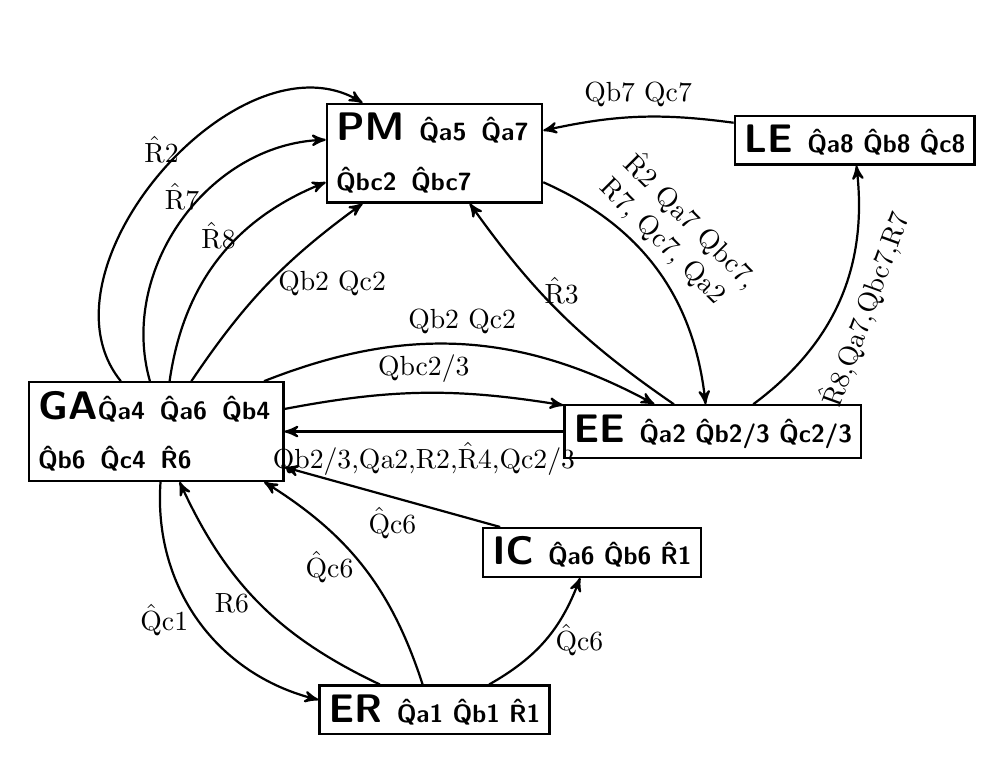
\begin{tikzpicture}[->,>=stealth',auto,node distance=5cm,
  thick,main node/.style={rectangle,draw,font=\sffamily\Large\bfseries}]
  \node[main node,text width=3cm] (ga) {GA{\small \^{Qa4} \^{Qa6} \^{Qb4} \^{Qb6} \^{Qc4} \^{R6}}};
  \node[main node] (ic) [below right of=ga,yshift=20mm,xshift=20mm] {IC {\small \^{Qa6} \^{Qb6} \^{R1}}};
  \node[main node] (er) [below right of=ga] {ER {\small \^{Qa1} \^{Qb1} \^{R1}}};
  \node[main node,text width=2.5cm] (pm) [above right of=ga] {PM {\small \^{Qa5} \^{Qa7} \^{Qbc2} \^{Qbc7}}};
  \node[main node] (ee) [below right of=pm] {EE {\small \^{Qa2} \^{Qb2/3} \^{Qc2/3}}};
  \node[main node] (le) [above of=ee,yshift=-13mm,xshift=18mm] {LE {\small \^{Qa8} \^{Qb8} \^{Qc8}}};

  \path (ic) edge node [below] {\^{Qc6}} (ga);
  \path (er) edge[bend right=20] node [right] {\^{Qc6}} (ic);


  %er <> ga
  \path (er) edge[bend right=20] node [left] {\^{Qc6}} (ga);
  \path (er) edge[bend left=20] node [left] {R6} (ga);
  \path (ga) edge[bend right=40] node [left] {\^{Qc1}} (er);


  %ga <-> ee
  \path (ga) edge[bend left=25] node [above] {Qb2 Qc2} (ee);
  \path (ga) edge[bend left=10] node [above] {Qbc2/3} (ee);
  \path (ee) edge[bend left=0] node [below] {Qb2/3,Qa2,R2,\^{R4},Qc2/3} (ga);

  %le <-> pm
  \path (le) edge[bend right=10] node [above] {Qb7 Qc7} (pm);
  %ee -> le
  \path (ee) edge[bend right] node [below,rotate=70] {\^{R8},Qa7,Qbc7,R7} (le);

  %pm <-> ee
  \path (ee) edge[bend left=10] node [above] {\^{R3}} (pm);
  \path (pm) edge[bend left=30] node [above,rotate=-45,text width = 2.5cm] {\^{R2} {Qa7} Qbc7, R7, Qc7, Qa2} (ee);

  %ga->pm
  \path (ga) edge[bend left=10] node [right] {{Qb2} Qc2} (pm);
  \path (ga) edge[bend left=80] node [above] {\^{R2}} (pm);
  \path (ga) edge[bend left=52] node [above] {\^{R7}} (pm);
  \path (ga) edge[bend left] node [above] {\^{R8}} (pm);
  \end{tikzpicture}
  \caption{A found-in-nature VTS. Nodes and edges are labelled with sets of molecules. \^{} indicates that the molecule is active.}
  \label{fig:mukund-vts}
\end{figure}

%%% Local Variables:
%%% mode: latex
%%% TeX-master: "main"
%%% End:


The figure~\ref{fig:mukund-vts} represent mammalian SNARE map
created by studying the wide array of literature.
% 
To construct the map, we have assumed that vesicles only contain a
single active v-SNARE, and we have attributed t-SNAREs and inactive
v-SNAREs that travel between compartments to one of the known vesicles
that go between the same source and target compartments.
%
In order to identify the active SNARE complex involved in any
particular vesicle fusion, we used two criteria.
%
The SNARE complex is formed \textit{in vivo}. In most papers, this is
determined by immunoprecipitation of the SNARE complex from the
relevant cell fraction.
%
Blocking SNARE complex formation (for example, using antibodies
against these SNAREs, or using cytosolic forms of these SNAREs) blocks
the specific transport step.
%
Note that these vesicles have been collected from multiple cell types, and
any given cell type is likely to contain only a subset of the vesicles in
the map.

In this figure, the rectangles represent compartments, the identities
of compartments are written within ER=endoplasmic reticulum,
ERGIC=ER-Golgi intermediate compartment, RE=recycling endosome,
EE=early endosome, LE=late endosome, LYS=lysosome, PM=plasma
membrane. The arrows represent vesicle edges.


% \ashu{Adopt }
% The set of SNAREs contained in these edges are written alongside each
% edge.
% %
% Actual names of these SNAREs are mentioned in the key
% alongside.
% %
% The red labels represent the paths taken by SNARES of the
% complex Stx-4-SNAP23-VAMP7.
% %
% Here, the cycles for two SNARE molecules,
% VAMP7 and SNAP23 are complete.
% %
% The green labels represent the paths
% taken by SNAREs of the complex Stx13-SNAP25-VAMP2.
% %
% Here the cycle for
% VAMP2 is complete. The blue labels represent the paths taken by SNARES
% of the complex Stx5-Gs28-Bet1/GS15-Ykt6.
% %
% Here, cycles for none of the
% SNAREs are complete.
% %
% So, even though most edges known so far are
% present in the map, paths for molecules (SNAREs) across the cell are
% still not complete.


\subsection{Yeast VTS}

\begin{figure}[t]
  \centering
  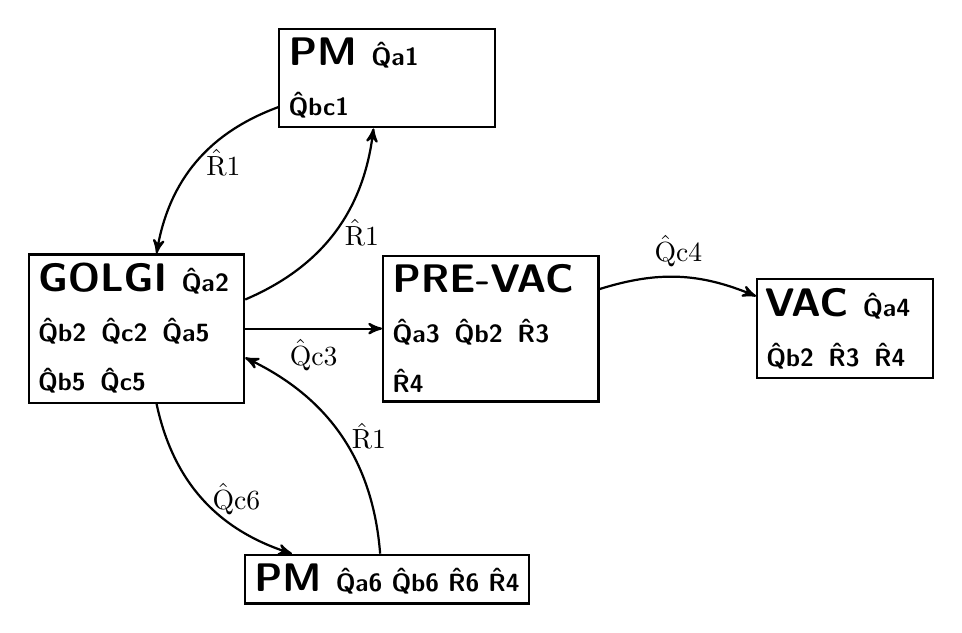
\begin{tikzpicture}[->,>=stealth',auto,node distance=4.5cm,
  thick,main node/.style={rectangle,draw,font=\sffamily\Large\bfseries}]
  \node[main node,,text width=2.5cm] (golgi) [] {GOLGI {\small \^{Qa2} \^{Qb2} \^{Qc2} \^{Qa5} \^{Qb5} \^{Qc5}}};
  \node[main node,text width=2.5cm] (pvac) [right of=golgi] {PRE-VAC {\small \^{Qa3} \^{Qb2} \^{R3} \^{R4}}};
  \node[main node,text width=2cm] (vac) [right of=pvac] {VAC {\small \^{Qa4} \^{Qb2} \^{R3} \^{R4}}};
  \node[main node,text width=2.5cm] (pm_up) [above right of=golgi] {PM {\small \^{Qa1} \^{Qbc1}}};
  \node[main node] (pm_down) [below right of=golgi] {PM {\small \^{Qa6} \^{Qb6} \^{R6} \^{R4}}};

  \path (golgi) edge[bend right] node [right] {\^{R1}} (pm_up);
  \path (pm_up) edge[bend right] node [right] {\^{R1}} (golgi);

  \path (golgi) edge[bend right] node [right] {\^{Qc6}} (pm_down);
  \path (pm_down) edge[bend right] node [right] {\^{R1}} (golgi);

  \path (golgi) edge[] node [below] {\^{Qc3}} (pvac);
  \path (pvac) edge[bend left=20] node [above] {\^{Qc4}} (vac);

  \end{tikzpicture}
  \caption{Yeast VTS}
  \label{fig:mukund-vts}
\end{figure}

%%% Local Variables:
%%% mode: latex
%%% TeX-master: "main"
%%% End:


In figure~\ref{fig:yeast-vts}, we present the yeast VTS.
%
We have borrowed the VTS from~\cite{burri2004complete}.
%
It has been adapted from the paper by
separating the v and the t SNAREs. 
%
It is clear that it is an incomplete description of the VTS.
%
For example, the inactive molecules were not reported in the reference.
%
We are currently searching for more literature that can help us complete
all known information about the VTS.
%


% It is important to note that it is not trivial collect all the information
% about such systems.

%%% Local Variables:
%%% mode: latex
%%% TeX-master: "main"
%%% End:


\end{document}

%--------------------- DO NOT ERASE BELOW THIS LINE --------------------------

%%% Local Variables:
%%% mode: latex
%%% TeX-master: "main"
%%% End:
